\documentclass[a5paper,french,openany]{memoir}
\usepackage[T1]{fontenc}
\usepackage[utf8]{inputenc}
\usepackage{tgpagella} %
\usepackage{mathpazo}  %
\usepackage{geometry}
\usepackage[round,sort&compress]{natbib}
\usepackage{url} %
\usepackage[hyperpageref]{backref} %
\usepackage[pagebackref]{hyperref}
\hypersetup{
  colorlinks=true, %
  urlcolor=purple,    %
  linkcolor=blue,  %
  citecolor=violet,   %
}
\usepackage{rotating}
\usepackage{bm}
\usepackage{indentfirst}
\usepackage{tocbibind}
\setcitestyle{aysep={}} 
\usepackage{amsmath}
\usepackage{amssymb}
\usepackage{eurosym}
\usepackage{amsfonts}
\usepackage{enumerate}
\usepackage{babel}
\usepackage{caption}
\captionsetup{labelfont=sc}
\def\frenchtablename{Tableau}
\usepackage{supertabular}
\usepackage{multirow}
\usepackage{tabularx}
\usepackage{float}
\usepackage{dsfont}
\usepackage{fancyvrb}
\usepackage{verbatim}
\usepackage{enumitem}
\usepackage{setspace}
\usepackage{comment}
\usepackage{subcaption}
\usepackage{graphicx}
\usepackage{tikz}
\usepackage{gensymb}
\usepackage{textcomp}
\usepackage{nameref}
\usepackage[bottom]{footmisc} %
\usepackage{tabulary}
\usepackage{tabularx}
\usepackage{booktabs}
\usepackage{fullpage}
\usepackage{morefloats}
\usepackage{makecell}
\usepackage{lscape}
\usepackage{pdflscape}
\usepackage{longtable}
\usepackage{rotating}
\usepackage{fancyhdr}
\usepackage{tocloft}
\usepackage{titletoc}
\usepackage{epigraph}
\usepackage{microtype} %
\usepackage[export]{adjustbox}
\usepackage[anythingbreaks]{breakurl} %
\usepackage{multicol}
\newsavebox\ltmcbox %
\renewcommand{\floatpagefraction}{.9}

\setlength{\fboxrule}{0pt}%
\setlength{\fboxsep}{10pt}

\newcommand{\BigWords}[1]{%
        \adjustboxset{min width=\linewidth, margin*=0.2em 1ex 0ex 0ex}%
        \foreach \i [count=\ni] in {#1}{%
                \ifnum\ni=1    
                        \adjustbox{}{\i}%
                \else
                        \\\adjustbox{}{\i}%
                \fi
        }\vspace{-1ex}%
}

\author{\huge{Adrien Fabre}%
} 

\title{
  \textcolor{white}{
  Un plan mondial pour le climat\\et contre l'extrême pauvreté
  } 
}

\date{} 

\begin{document}

\noindent\makebox[\textwidth][c]{
\fbox{%
\begin{minipage}{10cm}
  \vspace*{-3cm}
  \maketitle
  \vspace*{2cm}
\bfseries\sffamily
\BigWords{UN PLAN,MONDIAL,POUR LE CLIMAT,ET CONTRE L'EXTRÊME PAUVRETÉ}%
\vspace*{4cm}
\centerline{\today}
\end{minipage}}%
}%

\clearpage
\tableofcontents




\chapter*{Preface, by \textit{Gabriel Zucman}}\label{ch:preface}
\addcontentsline{toc}{chapter}{nameref{ch:preface}} 

How can we move towards a fairer world while effectively combating climate change~? This book proposes a clear and convincing solution that deserves to be widely debated.

The task is not an easy one. There are countless proposals to reduce greenhouse gas emissions, the inequalities of which are obvious. This failure to move forward together on the two major challenges of the 21st century --- combating climate change on the one hand, reducing economic disparities on the other --- has, for several decades, been at the heart of our collective inability to preserve the climate. 

Adrien Fabre's book is invaluable in demonstrating that this tension can be overcome. 

The most reliable instrument for tackling climate change is well known~: it consists of capping greenhouse gas emissions through a system of tradable quotas, the quantities of which must gradually decrease to reach zero shortly after the middle of the 21st century. 

By redistributing the revenues generated equally among all human beings (i.e., by allocating the same emissions permit to each inhabitant of the planet, a criterion of justice that is difficult to contest), this mechanism would make it possible to finance a universal basic income of around 50~euro{} per month per person between 2030 and 2060, thus eradicating the most extreme forms of poverty. 

A utopia~? Since completing his thesis, Adrien Fabre has specialized in opinion surveys on climate and redistribution. And this is where his treatise becomes fascinating. For his meticulous work overturns a commonly accepted idea~: that people in wealthy countries are hostile to international redistribution. <<~In reality, he writes, people are willing to embrace ecological change and solidarity - as long as the effort is international, equitably shared, and falls first on the wealthiest.~>>> 

It's not democracy that stands in the way of progress, it's the conservatism of economic elites and defeatism, for which this book is an indispensable antidote.

In fact, international transfers, although highly insufficient, are far from being completely negligible today~: on the order of 0.4 points of GDP for a country like France, or over 10 billion euros a year. There's nothing unrealistic about envisaging a doubling or tripling of these flows in the years to come. In fact, OECD countries have pledged to increase development aid to 0.7 points of GDP. The plan proposed by Adrien Fabre would result in international transfers of around 0.6~\% of global GDP, and would be in line with this trend. 

Proof of the urgency of the subject, initiatives to reconcile international economic justice and climate sustainability are multiplying. Nobel Prize-winning economist Esther Duflo estimates that the countries of the North should pay $500 billion a year to poor countries (0.5~\% of global GDP), just to compensate for the loss of human life caused by the current emissions of people living in industrialized countries. At the G20 Finance Ministers' meeting in São Paulo in February 2024, I presented a proposal for a coordinated minimum tax on the world's billionaires, which would, with a modest minimum rate of 2~\% on the wealth of the individuals concerned, raise at least 250 billion a year. It would be perfectly logical to allocate at least part of this revenue to the poorest countries, which, although home to relatively few billionaires, have made a powerful contribution to the enrichment of those in the North by giving them access to their markets. 

Adrien Fabre's book, based on the most recent research and his pioneering work, adds to this vital debate on the future of our planet. It is essential reading for all citizens committed to justice and progress.

\begin{flushright}
Gabriel Zucman
\textit{Professor at the Paris School of Economics and UC Berkeley}\\\
April 15, 2024
\end{flushright}

\chapter*{Motivation}{label{ch:intro}
\addcontentsline{toc}{chapter}{nameref{ch:intro}} 


A peaceful society, where everyone lives in dignity, where the conditions necessary for well-being are sustainably guaranteed for all~: this is the world we want to live infootnote{This preface takes passages from the introduction to my first essay, \textit{éloge de la naïveté} (unpublished, 2014), available at \href{https://adrien-fabre.com/elogeNaivete.php}{adrien-fabre.com/elogeNaivete.php}.}. Why do I think this book can help humanity evolve in this direction~? Because after ten years of studying economics and climate change, after completing a thesis on the conditions for the feasibility and acceptance of ecological moult, and focusing my academic research on opinions about climate and redistribution, my colleagues and I made a hopeful discovery. %
There is a solution to end global warming and extreme poverty, recognized by % of the world's population.
all the experts and supported by a majority worldwide. 
Although identified as early as 1990, this solution has not been discussed since.
since then. Indeed, it implies major North-South transfers, which the countries of the North have refused since the first climate negotiations. But the populations of these countries had not been consulted. And yet, by conducting representative surveys in 20 countries that account for three-quarters of the world's greenhouse gas emissions, it appears that this global solution to climate change would in fact be widely supported, even in the countries of the North. 
This promising result motivated me to bring this solution to life by writing this book and co-founding an advocacy association for the global redistribution of wealth, Global Redistribution Advocatesfootnote{To discover all our proposals, sign our petitions, join the association or make a donation~: \href{http://global-redistribution-advocates.org/}{global-redistribution-advocates.org}.}. %
We all want humanity to take charge, to organize itself 
to ensure that everyone has the necessities of lifeSurvey based on a representative sample of 499% of the population.
French survey I conducted in the fall of 2016, only 1~\% answered \textit{No} to the question~: \textit{Do you agree or disagree with the following statement? <<~I want humans to secure the conditions necessary for well-being: access to drinking water, food, healthcare, a healthy environment, safety, housing, education, information.~>>}}. 
Building on this common will, let's work together and overcome our disagreements.

To the best of my knowledge, no political party, association or think tank has ever proposed specific global redistribution measures. And yet, when I met with political leaders and associations, I realized that such proposals are received with interest, even enthusiasm. It seems to me that if current political proposals lack a global vision, it's because existing structures act like blinkers. Indeed, the institutions that structure political debate, such as voting and the media, operate on a national scale (at most). This national structure favors national measures and organizations. Another obstacle to global action is the tendency of individuals to cherish their families and friends, and to feel powerless and illegitimate to take action on a wider scale. %
Unfortunately, problems such as climate change and malnutrition cannot be solved without solidarity on a global scale. 

Our motivation to act for humanity is often bogged down by routine, personal worries or the inertia of social structures. %
But the most unbearable scourge holding us back is defeatism. It's the argument endlessly repeated~: <<~I agree with you, but people are too indifferent/selfish/skeptical/indoctrinated, leaders will never lead such a reform~>>. This reaction is the only one truly opposed to humanist proposals like those in this book. %
In reality, people are willing to embrace ecological change and solidarity, provided that the effort is international and equitably shared, and that it falls first and foremost on the wealthiest. %



The problem with defeatism is not that it is \textit{false}~: we can have real reasons to believe that humanity is %
The problem with defeatism is that it's bad for us. If we have found an obstacle on our road to happiness, we mustn't give up, but find mechanisms to remove it. Human beings accomplish wonders through perseverance, and self-censorship out of pessimism is the first step on the road to decline. 

defeatism %
is a pessimistic prediction of the future, with all its self-fulfilling aspects. It's an intellectual attitude which consists in thinking that, since the origin of life, predation has been the rule, and that it will continue to be so. It's thinking %
that society will reproduce its injustices and disasters. It's predicting the future as the arrival of what seems most likely to happen~: what already exists. This position is not only scientifically inaccurate~: we are not in a position to predict the future of human beings~; above all, it is morally very serious~: we must not predict our future, but choose it. %
We must therefore combine our efforts to maximize our chances of experiencing a future that satisfies our desires. In contrast to predicting the most likely future, we must choose the best possible future. But for this best future to take place, it's not enough to dream it lovingly; we need to understand the mechanisms by which we can bring it about, and the actions by which we can achieve it. In short, we need to build a project so that our future is in line with our hopes.
Within this project, I believe it is necessary to include a Global Plan for the climate and against extreme poverty. %

\chapter*{\textit{A day in the Burkinabe countryside}}\label{ch:narr_burkina}
\addcontentsline{toc}{chapter}{nameref{ch:narr_burkina}} 

It's 4 a.m. and roosters are waking the inhabitants of the small town of Houndé in Burkina Faso. Rosalie has just got up and is already walking towards the millet fields. Arriving at her plot, she places her baby under a tree and covers him with her scarf to protect him from the rain. It's sowing season, and a hard day's work awaits her. Rosalie alternates between spading and planting a seed, which she pushes into the earth while bending over. This year, she won't make it to the end of the field, as it has become too dry to cultivate. For lunch, Rosalie eats a millet cake that her daughter had prepared the evening before, topped with shea butter. As she sows, she can't help shedding a few tears as she thinks of her two children who left too young~: her eldest son, who died of lung disease after six months working in the Kiéré manganese mine, and her third, who died of malaria. At 8pm, night falls and Rosalie heads home. Apart from lunch, her energetic work was only interrupted to breastfeed. On the way home, she meets her neighbor, who tells her that two of his seven goats died last month after drinking downstream from the gold-mining area. She tells herself that she too must avoid this cyanide- and mercury-contaminated water when she goes gold-panning during the dry season. Arriving home, Rosalie dines with her husband and six children~: this evening, the family will share % of their food.
two eggs in addition to the daily tô with okra saucefootnote{Tô is a millet-based paste, and okra is a vegetable}. %
After the meal, Rosalie uses the water can to wash the dishes and do her ablutions, while her daughter studies by the light of their oil lamp. Rosalie is still hungry, but proud that the family has been able to buy her daughter a textbook by selling some of their millet reserves. As she lies down on her straw mat on the dirt floor, her back feels like it's been sawn in two --- alas, all the peasants here suffer such pain. Rosalie is looking forward to next week, when she'll be harvesting shea kernels with the women of her neighborhood. Not only will it be more fun than sowing, but with the sale of the almonds, she'll be able to buy a third hen and some dried fish. While her youngest son dances in the street with his friends to the sound of the radio, Rosalie drifts off to sleep, not even paying attention to the song extolling the virtues of water purification in a joyful mix of Mossi, Jula and French. 

\chapter{An unbearable status quo}}

Major scourges afflict humanity. In this book, we 
let's focus on two of them~: climate change and extreme poverty. The slow pace of progress in these areas is a disgrace for our society, which seems to care little for the vulnerable or for future generations. The situation is unbearable.

\section{Climate change}

The climate is a complex system, but the work of the IPCC has shown that we can approximate its evolution with a simple rule~: the rise in global temperature is proportional to the cumulative CO$_\text{2}$ emissions since the industrial revolution\footnote{Figure SPM.10 in \citet{ipcc_climate_2021} shows that one degree more corresponds to 2~000 GtCO$_\text{2}$.}. 
To put an end to global warming due to the accumulation of CO$_\text{2}$ in the atmosphere, we need to achieve carbon neutrality. In other words, we need to bring CO$_\text{2}$ emissions to zero. More precisely, emissions must reach zero, insofar as residual emissions can be offset by equivalent capture through reforestation or artificial carbon sequestration. The temperature at which humanity chooses to stabilize the climate determines the carbon budget, i.e. the emissions we have left to emit. For example, from 2024 onwards, humanity only has a budget of 1,000 billion tonnes (Gt) of CO$_\text{2}$ to have two chances in three%.
\footnote{Cf. Table SPM.2 in \citet{ipcc_climate_2021}. The use of a probability (<<~two chances out of three~>>) comes from the fact that climate models include a margin of error on the temperature reached by a given carbon budget.} to contain warming to +2\textdegree{}C. 
To meet this carbon budget, CO$_\text{2}$ emissions (currently 38~Gt per year) could be reduced by the same number of tonnes each year, until they reach zero in 2077.  %

If, on the contrary, emissions continue to rise, warming could reach +4°C by 2100, and up to +7-8°C between 2300 and 5000. Antarctic melting could raise sea levels by 15 metres by 2500 and submerge coastal areas where 340 million people currently live by 2100. In addition, areas home to nearly a billion people would be submerged by 2300}. Vast areas of China, South Asia and the Middle East would be rendered uninhabitable in the XXII$^\text{e}$ century due to a lethal combination of heat and humidity\footnote{\citet{pal_future_2016,im_deadly_2017,kang_north_2018}.}. Even in a less extreme emissions scenario, with a temperature of +2\textdegree{}C in 2100, sea levels would (in the absence of dykes) submerge areas where 190 million people currently live. %
If nothing is done to combat climate change, the population exposed to drought would triple by mid-century --- this exposure being particularly pronounced around the Mediterranean and in the Middle East. In addition, 4 billion more people would be exposed to malaria and dengue fever, as the mosquitoes that carry these diseases move up into previously temperate zones --- including Europe\footnote{\cite{colon-gonzalez_projecting_2021}.}. It is estimated that the increase in warming due to the emissions of a dozen Europeans during their lifetime causes additional death. Limiting global warming to 2°C would prevent 6 million annual deaths due to climate change by 2100 (as many as cancer deaths today)}. In the absence of adaptation measures, climate change will lead to a drop in agricultural yields of around 20~\% by mid-century for the main crops in sub-Saharan Africa. A warming of 2 or 3 degrees Celsius, on the other hand, would lead to a drop in agricultural yields against which even adaptation measures would be ineffective. Generally speaking, our settlements, land uses and infrastructures are adapted to the current climate. Climate change will render many of them obsolete, if not simply destroyed. 

To sum up, continued greenhouse gas emissions would jeopardize many parts of society, multiplying droughts and floods, reducing agricultural yields, increasing the likelihood of violent conflict, and leading to major population displacementsfootnote{This paragraph repeats elements of the preamble to my thesis \citep{fabre_is_2020}, and is based on numerous works \citep{cattaneo_human_2019,carleton_social_2016,dell_temperature_2012}.}. 


\section{Extreme poverty} %

The World Bank defines extreme poverty as consumption of less than 2~\textit{\texteuro{}} per day (adjusted for the cost of living). The 2~\textit{\texteuro{}} threshold (2.15~\textit{\$} in constant 2017 dollars, to be exact) is expressed in purchasing power parity~: it corresponds to what 2.15~\$ can buy in the United States. In a country like India, it takes less than $1 to buy products that cost $2.15 in the United States. Throughout the book, we use \textit{\$} (in italics) to denote the dollar in purchasing power parity (PPP) terms, and \$ to denote the nominal dollar. Similarly, we will denote the euro in PPP terms by \textit{\teuro{}} and the nominal euro by \euro{}). %
This threshold is sufficient to meet minimum nutritional needsfootnote{\citet{allen_absolute_2017} calculates that, in low-income countries, the extreme poverty threshold allows us to afford 3 m² in a home heated to 15textdegree{}C and a diet consisting solely of oil and a cereal (sometimes supplemented by lentils), which provides a daily intake of 2100 kcalories, 50 g of protein and 34 g of fat.}. 
The number of people living in extreme poverty overlaps with the 700 million undernourished people in the world, according to the World Bank. 

Although the proportion of people living on less than 2~\textit{\texteuro{}} a day has been divided by four in the last thirty years, extreme poverty still affects two-thirds of the population in a country like Malawi. In fact, with population growth, there are more Africans living in extreme poverty today than there were thirty years ago. If extreme poverty has been reduced over the period, it's only thanks to the development of Asia, and China in particular. %

\begin{figure}[h!] 
  \caption[Inequalities in GDP per capita]{GDP per capita relative to the world average, adjusted for cost of living (2022, World Bank). %
  }label{fig:GDPpc}
  \makebox[\textwidth][c]{\includegraphics[width=.56\textwidth]{../figures/policies/GDP_pc_PPP_en.pdf}}%
\end{figure}

China's GDP per capita is now around the world average, at 1~000~euro{} per month, according to the World Bank (2022). %
In comparison, GDP per capita is three times higher in high-income countries and ten times lower in low-income countries (Figure \ref{fig:GDPpc}). It's hard to exaggerate the gap in living standards between countries. In fact, a transfer of just 1~\% of GDP from high-income countries %
would mechanically double average income 
low-income countries, home to 700 million people%.
\footnote{
Of the 26 low-income countries, defined by GDP per capita %, the following are of particular interest.
below $1~135~\/year, 22 are in sub-Saharan Africa and 4 outside (Afghanistan, North Korea, Syria and Yemen). 1.2 billion people live in a high-income country (with a GDP/capita of over $13~845~\/year).
}. %

\section{The link between climate and poverty} 

Anyone who cares about the well-being of human beings wants to put an end to poverty. 
Similarly, it is not necessary to attach any intrinsic value to Nature or biodiversity in order to fight climate change~; it is sufficient to be concerned about human well-being. Climate change jeopardizes the living conditions of large sections of the population, not only for future generations, but also right now, %.
particularly in tropical countries. Indeed, global warming is all the more problematic in areas that are already hot --- and home to most of the world's poor ---, as these areas are more exposed to drought, lower agricultural yields, and the difficulty of working outdoors (or without air conditioning). While the poorest are bearing the brunt of climate change, they also lack the means to cope with it~: %
they don't have the resources to buy an air conditioner, build a dyke or migrate to an unscathed area. Not only does poverty increase vulnerability to climate change, climate change also increases the risk of poverty. It is estimated that between 32 and 132 million people will fall into extreme poverty by 2030 as a result of climate change (particularly through its effects on health and agricultural commodity prices). By reducing growth in the poorest countries, climate change increases inequality~: it is estimated that the income gap between the richest and poorest countries has already increased by 25~\% as a result of climate changefootnote{\cite{diffenbaugh_global_2019,khalfan_climate_2023}.}. %


Climate change raises the question of the global and temporal distribution of power and wealth. %
Indeed, the distribution of greenhouse gas emissions is extremely uneven~: while the richest 1~% of Americans emit an average of 318~tCO$_\text{2}$e per year, the average Indian emits 2~t and the poorest 10~% of Rwandans emit just 0.1~t\footnote{The concept used here is the carbon footprint, i.e. the emissions attributable to individual consumption, both direct (such as petrol consumption) and indirect (the emissions involved in producing the products consumed).}. %
Globally, the top 1~\% are responsible for 50~\% more emissions than the bottom half of humanity. 
And unlike many poor Africans or South Asians who have yet to be born, wealthy, elderly Westerners with large carbon footprints are unlikely to suffer much from climate change, and therefore have little interest in changing their opulent lifestyles, As shown by vulnerability indices \citep{chen_university_2015} or estimates of climate change damage as a function of country GDP \citep{burke_global_2015}.}. 
So, to prevent the dramatic impacts of climate change, it is misleading to frame the question simply in terms of temperature, %.
because the heart of the problem lies in the inequalities between human beings who differ in terms of wealth, location or generation. As such, a solution to climate change or its impacts can only be coherent if it is equitable, and therefore involves a substantial transfer of resources from today's rich to tomorrow's poor. %


\chapter{The need for global redistribution}}

\section{A moral prescription}
Whether religious, philosophical or intuitive, morality generally prescribes transfers from high-income earners to low-income earners, and therefore from high-income countries to low-income countries. This is the case with utilitarianism, the reference ethical theory used in economics. Utilitarianism attributes the same weight to each person, and thus justifies the transfer of one euro from a rich person to a poor one, since one euro will bring more satisfaction to the latter. According to the theory of optimal taxation, this reasoning is valid as long as an increase in taxes does not encourage the richest to expatriate, conceal or reduce their activity to the point of diminishing the revenues obtained. Economists have calculated the optimal tax system taking these effects into account. In these calculations, \citet{kopczuk_limitations_2005} are limited to a single rate (a \textit{flat tax}) and do not allow for a progressive scale. Without this restriction, the true optimum would be even more redistributive}. %
The theory of optimal taxation can only rationalize the current situation by turning moral on its head. Indeed, researchers have shown that the virtual absence of international transfers is only optimal if we assign a value 2~000 times higher to an American than to a Congolese (or, alternatively, if we assign a value 100 times higher to the American and consider that only one-twentieth of the money transferred will reach its recipient, the rest being diverted by corruption). %

\section{A legal-diplomatic commitment}
Beyond ethical considerations, the imperative of global redistribution has legal foundations. In 2015, all countries adopted the Sustainable Development Goals (SDGs), at the forefront of which is the elimination of extreme poverty by 2030. Yet low-income countries do not have sufficient domestic resources to eliminate extreme poverty. Indeed, in the poorest countries, expropriating all incomes from 7~\textitteuro} a day would not be enough to finance sufficient transfers to lift their inhabitants above 2~\textitteuro} a day by 2030.\footnote{Cf. \citet{fabre_shortfall_2024}.} %
In other words, it's impossible to achieve the first MDG without international transfers. And this, while the first MDG is limited to ensuring an income barely sufficient to avoid hunger. The transfer needed for this first MDG corresponds to 0.1~\% of global GDP, or as much as is spent on pet food. footnote{Cf. \href{https://www.grandviewresearch.com/industry-analysis/pet-food-industry}{grandviewresearch.com/industry-analysis/pet-food-industry}.}. %

To ensure a decent life, which guarantees access to water, sanitation, education, a health system and a minimum ability to move about and socialize, it is estimated that an income of at least €7 per day is required. 
620 million people live in a country where GDP per capita is below this threshold, and where it is therefore strictly impossible to ensure a decent life for everyone by mobilizing domestic resources alone. 
In total, half of the world's population lives below the poverty line, according to \href{https://ourworldindata.org/grapher/distribution-of-population-between-different-poverty-thresholds-up-to-30-dollars}{ourworldindata.org}.}. Closing the gap between them and this threshold would cost 2~\% of global GDP in 2030footnote{In purchasing power parity, this gap (the \textit{poverty gap}) is 4~800 billion dollars, or 3.4~\% of global GDP of 140~000 billion. Assuming annual world growth of 3.5~\% (the rate observed over the last 20 years), we find %.
2.1~\% of world GDP in 2030.}. %

In 1970, industrialized countries pledged to allocate 0.7~\% of their GDP to official development assistance, including 0.2~\% of GDP for the least developed countries. This commitment, renewed in 2005 and 2015, has never been fulfilled. In fact, actual aid amounts to only half of the aid promised, including only 0.06~\% for the least developed countries, and only a handful of countries are meeting their commitments: Luxembourg, Sweden, Norway, Germany and Denmark. 
\citep{oecd_oda_2023}.}. 
It is estimated that the bulk of the SDGs could be achieved if industrialized countries finally honored this commitment. To achieve a maximalist version of the SDGs (including ensuring access to clean energy) or another ambitious target in relation to the status quo (such as ensuring 7~\textit{\texteuro{}} per day for everyone), high-income countries would need to transfer more resources, probably between 2 and 5~\% of their GDP.%.



\section{An imperative for decarbonization in the South}

Lastly, a climate justice solution would have to be supported even by someone who would not feel bound by ethics or international commitments and would only care about the climate out of concern for the environment.  
his well-being and that of his descendants. Indeed, to put an end to climate change, %.
the whole world needs to decarbonize. 
However, international transfers are a prerequisite for low-income countries to decarbonize. On the one hand, these countries have other priorities than decarbonization, and therefore deploy the most affordable energy system --- often based on coal. On the other hand, these countries argue --- and rightly so --- that they are the most vulnerable to climate change and have contributed only marginally to it. Africa and South Asia combined are responsible for 6~\% of cumulative CO$_\text{2}$ emissions. %
}. In international negotiations, these countries generally announce two emission reduction targets: an unconditionally unambitious target and an ambitious target conditional on external financing. For example, Ethiopia has pledged to unconditionally reduce its emissions by 14~\% by 2030 compared with a no-climate-action scenario, and is making a 69~\% reduction conditional on $250 billion in financing. %
At the same time, developing countries (supported by the UN General Secretariat) are calling for annual transfers of $100 billion to compensate for the loss and damage to the climate caused by emissions from developed countriesfootnote{Cf. \cite{tc_proposal_2023,sgnu_bridgetown_2023}.}. While experts estimate that the transfers required would be two to four times this amount, only 700 million were \textit{promised} in 2023 at COP 28%.
\footnote{Cf. \cite{songwe_climate_2023,markandya_integrated_2019,robinson_valuing_2021} and \href{https://www.theguardian.com/environment/2023/dec/06/700m-pledged-to-loss-and-damage-fund-cop28-covers-less-than-02-percent-needed}{www.theguardian.com/environment/2023/dec/06/700m-pledged-to-loss-and-damage-fund-cop28-covers-less-than-02-percent-needed}%
.}.

More generally, the international arena is tending to polarize between the South, which is demanding a fairer world order, and the North, which is reluctant to give up its dominant position. For example, the African Union recently called for a global carbon pricing regime, a tax on financial transactions and a reform of the financial system, in order to benefit from dedicated, affordable and sustainable climate financing, dissociated from national and geopolitical interests. Southern countries are also critical of international negotiations on corporate taxation, which are taking place under the aegis of the OECD and exclude many low-income countries. In November 2023, although the OECD countries voted against it, the countries of the South pushed through a resolution at the UN establishing a Convention on International Tax Cooperation (akin to the climate COPs). Southern countries hope that this negotiating framework will be more favorable to their interests than the OECD. 

Despite the tendency of countries in the North to defend their short-term financial interests, there is hope that they will accede to certain demands from the South. 
Whether in defense of humanist values or to restore its often tarnished image, 
the West seeks to present itself as a model based on human rights, democracy and sustainable development. 
For example, Ursula von der Leyen, President of the European Commission, recently came out in favor of global carbon pricingnote{Cf. her \href{https://twitter.com/vonderleyen/status/1700416700238225659}{Tweet} of September 9, 2023.}, and a working group on international taxation (including carbon) was launched in December 2023 jointly by France, Kenya, Spain and Barbadosnote{Cf. \href{https://www.elysee.fr/admin/upload/default/0001/15/91b013291db03bcc5f2f6b84de39a81ae0c04c7d.pdf}{https://bit.ly/taskforce\_tax}.}. 

Humanist values would at last be properly defended in the event of an international climate agreement and fair taxation that would involve the countries of the North. Such an agreement would have the potential to rebuild geopolitics on sound foundations and pacify international relations. Conversely, it has been shown that climate change increases the risk of armed conflict, particularly in Africa.

In the next chapters, we propose a Global Plan to end climate change and extreme poverty, involving major North-South transfers, while being accepted by %.
the populations of Northern countries.




\chapter{The heart of the Global Climate Plan}}

We saw in Chapter \ref{ch:statu_quo} that humanity has a carbon budget that must not be exceeded to keep global warming below a given target. The Paris Agreement sets this target. Signed by all countries in 2015, it aims to contain warming <<~nettly below 2\textdegree{}C (...) by continuing the action taken to limit temperature rise to 1.5\textdegree{}C~>>. \\

How can we guarantee an emissions trajectory in line with this carbon budget~? 

The safest approach would be to cap global emissions, with an annual cap that decreases in line with the target. \\

How then to allocate the CO$_\text{2}$ emissions allowed~? 

The simplest %.
is to allocate the same emissions permit to each human. \\

Should the resale of emissions permits be authorized? 

Yes, %
Setting up a carbon market is preferable to a system of non-tradable individual carbon quotas for several reasons, detailed in the Frequently Asked Questions (FAQ, p. \pageref{q:rationing}). In particular, the market is more favorable to the most modest, as it provides financial compensation to those who do not use up all their quota.

These three answers suffice to grasp the essence of the Global Climate Plan.

\paragraph{Preventing misunderstandings}
It is important to understand that by introducing a cap on emissions, global emissions are by construction equal to this cap, thanks to mechanisms (detailed in Sections \ref{sec:pcp_quota} and \ref{sec:implementation}) that prevent it from being exceeded. This is the main interest of this Plan.

This cap settles the temperature issue, %.
but not the social question~: it's the distribution of emissions permits that determines how efforts are shared. The egalitarian distribution we propose will bring about a major North-South redistribution and put an end to extreme poverty. 

To avoid common confusion, it should be noted from the outset that this system would not allow carbon offset credits to be purchased through reforestation projects. The proposed system resembles the European carbon market in place since 2005, but is radically different from the dysfunctional and greenwashing carbon offset market. The European market caps emissions from the industry and electricity sectors, on a trajectory that decreases to zero by 2040. It will be supplemented in 2027 by a second carbon market covering emissions from transport and buildings. These carbon markets should not be confused with the carbon offset market, which allows companies or individuals to buy carbon credits to offset their emissions through projects (such as reforestation) in developing countries. Carbon offsetting is problematic because it does not guarantee a reduction in global emissions. Indeed, it is not clear whether the projects financed result in a \textit{permanent} reduction in emissions (for example, an area reforested during the project may be deforested later) and \textit{additional} (for example, a forest could have grown back even in the absence of financing, or reforestation in one place may generate \textit{carbon leakage} by causing deforestation in another). For these reasons, carbon credits are not eligible on European carbon markets. Carbon credits actually reduce European emissions}.



\paragraph{Functioning}
The system outlined above can be implemented as follows. Each year, a limited number of emissions permits are created, in line with the emissions trajectory set. These emission permits are auctioned to the companies at the source of the CO$_\text{2}$ emissions, and in particular to those who market % of their emissions.
coal, oil or gas. These companies must purchase permits corresponding to their emissions. Finally, the revenue generated by the sale of permits is redistributed as an equal basic income for all human beings. 

\paragraph{Who pays~? Who receives~?}
The basic income is equal to the revenue generated divided by the population. The revenue generated is equal to the price of carbon multiplied by global carbon emissions. Thus, the basic income is equal to the price of carbon multiplied by the average human carbon footprint. 

Although, for practical reasons, we would distribute money rather than emission permits to individuals, these two options are equivalent. Let's imagine that every human being received the same emission permit and could sell it to polluting companies on the carbon market. The amount he or she would receive would be equal to the price of carbon multiplied by the individual quota, i.e. exactly the basic income. In this way, there is a perfect match between egalitarian allocation of emissions permits and egalitarian allocation of revenues. %

Even if it would be advantageous %.
to assert that the price of carbon is paid by polluting companies, it is more accurate to explain that it is consumers who bear the cost. 
This is because polluting companies pass on the cost of emission permits in the form of higher prices, so that each individual faces a higher expense, equal to the price of carbon multiplied by his or her carbon footprint. As a result, the basic income barely covers the price of carbon paid for an individual whose carbon footprint is equal to the world average. Individuals with a carbon footprint higher than the world average lose purchasing powerfootnote{This result stems from assumptions justified in Appendix \ref{app:indiv}. The carbon footprint and its global average mentioned are those \textit{after} the Plan comes into force.
}. Conversely, people with a low carbon footprint gain. In other words, the proposed system operates a global redistribution from the polluters to the frugal --- so, to a first approximation, from the rich to the poor. 

To find out more, the FAQ (p. \pageref{q:riches}) contains justifications for this system compared to others, explaining how it is favorable to the most modest and would force the rich to reduce their emissions.


\paragraph{Tax or quota~?}
In conclusion, this system sets a quantity~: the regulator sets an emissions quota and lets the market determine the carbon price. Conversely, we could imagine a carbon tax~: the regulator sets the price and lets the market determine emissions. Provided that the price of carbon is the same in the system that sets the quantity and the one that sets the price, the two systems are strictly equivalent (they result in the same emissions priced at the same level). Our proposal is based on a system that fixes the quantity, since the primary objective is to respect the carbon budget (and fixing the price does not make it possible to forecast emissions accurately). The FAQ (p. \pageref{q:taxe}) explains this further. 


\paragraph{Conclusion}
To sum up, we can put an end to global warming by capping emissions, and eliminate extreme poverty with a basic income. A simple and effective system for dealing with both problems is to combine these two solutions. This is the heart of the Global Climate Plan, %.
which constitute the first two principles detailed in Chapter \ref{ch:principes}. For reasons of justice and geopolitics, a few adjustments are necessary to complete our proposal~: I also describe them in Chapter \ref{ch:principes}. %
Finally, this Global Climate Plan must be complemented by other measures%.
~: I outline them in Chapter 1.


\chapter*{\textit{A day at Poitiers hospital}}\label{ch:narr_poitiers}
\addcontentsline{toc}{chapter}{nameref{ch:narr_poitiers}} 

Catherine is a nurse at Poitiers University Hospital. Today, she baked cakes to celebrate the end of construction work with her colleagues~: now that the hospital has been renovated, there's no more drilling noise and, above all, no more unbearable temperatures during the summer months. Catherine, on the other hand, didn't wait for the Global Plan to raise the price of gas %.
to renovate her house. When she inherited the house in 2028, the energy audit revealed that, given the anticipated price rise, the most economical option for heating was to insulate the walls and attic, and replace the oil-fired boiler with a heat pump. Repaying the works costs Catherine a little less than she would have spent on fuel oil, and by the time she finishes paying off her loan in 2041, she'll really be making up for lost time. 

In her well-to-do hamlet of Charassé, almost everyone has an electric car. Catherine opted for an electric scooter when she got rid of her old Twingo. She made this choice to be able to finance her daughter's business school~: doing without a car saves a lot of money, especially with the rising price of petrol. And she doesn't miss the traffic jams. Even if she was apprehensive about no longer doing her shopping by car, she likes having it delivered after all. In fact, the most annoying thing is when she goes on vacation with her youngest child. Whereas it used to take her two hours to drive to her parents' home in Les Sables-d'Olonne, it now takes her six hours door to door~: one bus then three trains. That's when she can't find a carpool. Thanks to the alert she's set up, she still manages to spend weekends at her parents' as regularly as before. She jumps at the chance when a driver makes a round trip similar to hers, and sometimes makes some nice encounters. Last time, she had a crush on her driver~: a former worker at the closed-down aircraft engine factory, now a solar panel installer. Thinking back to his angelic smile and sun-kissed complexion, Catherine really hopes to bump into him again on the next trip.


\chapter{A widely supported Plan}}

In addition to this book and a YouTube videofootnote{The video summarizing the book in 30 minutes is available at \href{https://bit.ly/CH_GCP}{bit.ly/CH\_GCP}.}, other volunteers and I are advocating the Global Climate Plan to multiple stakeholders through the advocacy association we founded, \textit{Global Redistribution Advocates}. %
Our motivation to defend this Plan stems from the results of my academic research. Since my thesis, I have specialized in opinion surveys on climate and redistribution. I conducted an international survey in 20 countries on attitudes towards climate policies, and a complementary survey in the USA and Europe on opinions towards the global redistribution of wealth. Although the idea at the heart of the Global Climate Plan --- a global carbon quota with egalitarian redistribution of revenues --- is long-standing and considered the canonical climate policy by economists, no survey had tested this proposal with public opinion. Surveys, however, reveal majority support worldwide. What's more, various survey methods indicate that support is sincere and could materialize electorally. 
It's this new element --- the fact that the public supports such a Plan, even in countries that would lose out financially --- that justifies putting this idea back on the international negotiating table, and giving it serious consideration. In this chapter, I'll describe the history of the idea, followed by the results of opinion surveys.


\section{An old idea} 

\subsubsection{The genesis of the idea}
The polluter pays principle is a basic idea in economics, dating back to \citet{pigou_economics_1920}. The principle consists in making the person who causes external costs (in this case, the damage caused by climate change) pay for them (in this case, the greenhouse gas emitter). This can take the form of a quota market or a tax. The cost to the polluter encourages him to reduce his activity or make it less polluting, as these alternatives are now comparatively less costly. %
Furthermore, the revenues generated by pollution pricing must be spent in the most beneficial way possible for society.  
In the case of climate change, the simplest solution is probably to share the revenues equally. This egalitarian sharing can thus be conceived as an equal emissions permit for each human. 

Given this theoretical framework, it's hardly surprising that a global carbon quota distributed on an egalitarian basis has emerged as the canonical solution to climate change ever since it first emerged into public debate. It would appear that it was Michael Grubb, a professor at University College London, who first advocated this solution when the first IPCC report was being drafted in 1990. In his article, Grubb writes that <<~by far, the best combination in terms of long-term effectiveness, feasibility, equity and simplicity is achieved through a system based on tradable carbon emission permits, allocated on the basis of the same permit for each adult~>.>footnote{The original quote from \citet{grubb_greenhouse_1990} is <<~\textit{by far the best combination of long-term effectiveness, feasibility, equity, and simplicity, is obtained from a system based upon tradable permits for carbon emission which are allocated on an adult per capita basis}~>>.}. A year later, Anil Agarwal and Sunita Narain, of New Delhi's Centre for Science and Environment, published a seminal text on climate justice that advocated much the same solution, while castigating the <<~environmental colonialism~>> of developed countries. %
Since then, many have expressed their support for such a solution~: \citet{bertram_tradeable_1992,baer_equity_2000,jamieson_climate_2001}, or more recently the report \citet{blanchard_major_2021}\footnote{<<~Le Nord devrait
frankly acknowledge its responsibility for future climate damage, and
consider the possibility of paying the South for the implementation of investments
necessary to green its economy. This could be achieved by asking the countries of the South to
market] mechanism and offering them free permits in proportion to their population, which would at the same time increase incentives for mitigation in developing countries.
} (former IMF Chief Economist and <<~Nobel~>> Prize winner, respectively) and \citet{rajan_global_2021} (former Governor of the Indian Central Bank and IMF Chief Economist). 

\subsubsection{The failure of climate negotiations}
Alas, \citet{bertram_tradeable_1992} reports that diplomats from wealthy countries such as the USA and Japan evacuated this option from climate negotiations as early as 1990. At the 1992 Earth Summit, George Bush made it clear that his administration was not prepared to make any contribution to the rest of the world with his now-famous phrase~: <<~the American way of life is not negotiable~>>\footnote{The original quote is <<~The American way of life is not up for negotiation~>>.}. %
As texts must be adopted unanimously, the UN framework has always sought a consensual solution. In the 1990s, proposals involving large-scale international transfers were rejected by countries such as the United States, while developing countries refused to accept any binding targets in the absence of such transfers. In 1997, negotiations on the Kyoto Protocol resulted in national targets for developed countries only. This division into two categories of countries turned the Kyoto Protocol into a stalemate~: emissions from developing countries were not limited, while developed countries only agreed to a small reduction in their emissions (not to mention the United States, which demanded that developing countries contribute and therefore never ratified the Protocol). To break the deadlock, diplomats meeting in Copenhagen in 2009 sought to negotiate a differentiated emissions reduction for each country. Developed countries put unilateral emission reduction commitments on the table, along with a promise to contribute $100 billion annually (less than one thousandth of global GDP). However, developing countries considered these commitments insufficient (the least developed countries, for example, called for a contribution of at least 1.5~% of developed countries' GDP) and refused to make binding commitments. As a result, no agreement was reached in Copenhagen. Since then, ambitions have been scaled back. The Paris agreement signed in 2015 had the merit of ratifying a universal objective for limiting temperature rise, but it also formalized the transition to a non-binding regime in which each country voluntarily defines its contribution in terms of emissions reductions. 

Not only are the targets set by each country insufficient to achieve the Paris Agreement objective, but the policies implemented are also likely to miss these targets. Thus, the policies and actions 
current trends point to a warming from 2.6\textdegree{}C to 2.9\textdegree{}C by 2100footnote{Cf. \href{https://climateactiontracker.org/global/temperatures/}{climateactiontracker.org/global/temperatures}.} and a temperature that would continue to rise at an alarming rate after 2100. 

In the light of the history of climate negotiations, two elements seem to me to be essential to obtaining a binding agreement on emissions reductions~: substantial North-South transfers (of the order of 1~\% of world GDP) and the abandonment of the aspiration to universality (the United States having always refused any binding agreement, to name but one).

\subsubsection{Ever-growing support from economists}
In a book entitled <<~Global Carbon Pricing: The Path to Climate Cooperation~>>\footnote{\citet{cramton_global_2017}.}, a number of experts, including three <<~Nobel~>>prizewinning economists (Joseph Stiglitz, Jean Tirole and William Nordhaus), take turns extolling the merits of global pricing of CO$_\text{2}$ emissions. In this book, \citet{gollier_negotiating_2015} set out the various possible options for distributing the revenues from this pricing system according to a generosity parameter, and describe the egalitarian allocation of revenues as being the most generous towards the most disadvantaged}. The least generous allocation being that (known as \textit{grandfathering}) where revenues are allocated in proportion to emissions}. 
In another chapter, \citet{cramton_international_2015} assume that each state defends its national interest and propose the following agreement between the countries %.
proactive. %
The generosity parameter would be chosen by countries with per capita emissions around the world average, and then the climate ambition would be set at the minimum level proposed by the participating countries, although we could adapt their proposal to a cap-and-trade system by setting the carbon budget. I therefore prefer to use the more general term \textit{climate ambition}.}. As countries with average emissions are little affected by the international transfers implied by the agreement, they would strategically choose the parameter of generosity that would maximize climate ambition~: neither too high, so that rich countries propose a high level of ambition, nor too low, so that poor countries gain and subscribe to a high level of ambition. \citet{van_den_berg_implications_2020} propose a <<~two-pronged transition to global carbon pricing~>>~: a \textit{climate union} that would merge existing permit trading systems and gradually integrate new ones, and a reorientation of international negotiations (the COPs) to determine the rules of global carbon pricing and the level of generosity. The \citet{fmi_how_2019} also supports global carbon pricing and, in the short term, a carbon price floor. To move towards climate justice, the institution proposes either differentiated prices between countries, or the solution we defend~: a uniform price with international transfers. 

Support for global carbon pricing is not confined to economists \textit{mainstream}~: it is also backed by environmental economists who favor degrowth. For example, a system equivalent to the Global Climate Plan (called \textit{cap and share} by \citealp{douthwaite_degrowth_2012}) is the first of six policy measures proposed in \textit{the economics of degrowth} by \cite{kallis_economics_2012}. Similarly, heterodox economists such as Elinor Ostrom and Robert Costanza advocate a variant of global pricing, where half of the revenues would fund a basic income and the other half low-carbon projectsfootnote{barnes_creating_2008}.%.

\section{A recent discovery~: public support} \label{sec:support}

In international negotiations, diplomats seem to defend short-term national interests rather than climate justice. 
But do their attitudes correctly represent the values of their peoples~? 
Surprisingly, it's only recently that opinion polls have taken up the issue. All converge in finding broad support for a global, redistributive climate policy. Before presenting in detail the results of surveys carried out by my colleagues and myself examining attitudes towards the Global Climate Plan in 20 countries, %.
Let's take a look at other surveys dealing with similar issues. 

\subsection{Support for global climate policies}

Over the past dozen years, a series of academic studies have focused on revealing preferences in terms of the distribution of the decarbonization effort between countries. These studies cover many countries, using representative surveys of the population. While the various studies are difficult to compare, as they differ in their approach and the way they ask the questions, two regularities stand out. Whatever the country in which the survey is carried out, the preferred options are those in which the decarbonization effort is universal, and those that appear egalitarian. For example, \citet{carlsson_is_2011} find that Swedes prefer all countries to be allowed to emit the same amount of emissions per capita. In a survey of the USA, Germany, France and the UK, \citet{bechtel_mass_2013} reveal that a climate agreement is most preferred when it includes a large number of countries, %.
and less appreciated if rich countries are the only ones to bear the decarbonization effort compared to the option where <<~rich countries pay more than poor countries~>> or where countries <<~pay in proportion to their emissions~>>. Similarly, \citet{carlsson_fair_2013} highlight that the option least appreciated by the United States or the Chinese is that where low-emission countries are exempted from any effort, while in a survey covering 28 countries (including the most populous), a large majority agree that all countries should contribute to reducing emissions \citep{dabla-norris_public_2023}. 
\citet{schleich_citizens_2016} report an identical ranking of options in China, the USA and Germany, with a preference for the polluter-pays principle followed by consideration of ability to pay, and last place for the option where countries that pollute the most have more permits to pollute. The authors also find that only 13 to 28~\% of people (depending on the country) consider their personal position adequately represented in international negotiations~; and 73 to 87~\% think that the fight against climate change requires new international treaties. Finally, \citet{meilland_international_2023} find that the principle preferred by the French and the Americans is that <<~all countries commit to converging towards the same average per capita emissions, compatible with controlled climate change~>>.}. %

Furthermore, the surveys all reveal strong support for the fight against climate change. For example, in a large-scale survey of 125 countries covering 94~\% of the world's population, \citet{andre_globally_2024} find that 89~\% of humans want a more ambitious climate policy, and 69~\% are willing to contribute 1~\% of their income to fighting climate change (a value which is a credible estimate of the cost of decarbonization). 
On the other hand, 81~\% underestimate the proportion of the population willing to contribute~: %.
This share is perceived on average at 43~\%, 26 points lower than the reality. This underestimation (known as "pluralistic ignorance") of environmental concerns may explain the lack of ambition in international climate agreements. %

While most surveys investigate general or theoretical issues, very few have tested adherence to well-defined global climate measures. In fact, apart from my own studies, I know of only one, published in the scientific journal \textit{Nature}. In this five-country survey, \citet{carattini_how_2019} test different variants of a global carbon tax. For the variant with egalitarian redistribution of revenues, they find support close to 50~\% in high-income countries (USA, Australia, UK) and South Africa, and over 80~\% support in India. These results are consistent with those of the surveys I have collaborated on, detailed in \citet{fabre_international_2023} and summarized below. 

\begin{figure}[b!] %
  \caption[Support for global climate policies]{Support for global climate policies} 
  \makebox[\textwidth][c]{\includegraphics[width=paperwidth]
  {../figures/OECD/Heatplot_global_tax_attitudes_share_en.pdf}}\label{fig:oecd} %
  {\footnotesize $\quad$ Note 1~: Percentage of responses \textit{Very} and \textit{Somewhat Favorable}, excluding responses \textit{Indifferenttextperiodcentered{}e} ($n$ = 40,680). Source~: \citet{fabre_international_2023}. %
  Blue denotes a relative majority. %
  \\ Note 2~: *In Denmark, France and the United States, questions with an asterisk were asked differently. %
  } 
\end{figure}

The first of these surveys was carried out in 20 countries %.
between 2021 and 2022\footnote{With my co-authors Antoine Dechezleprêtre, Tobias Kruse, Bluebery Planterose, Ana Sanchez-Chico and Stefanie Stantcheva, we conducted a survey on attitudes towards climate change and climate policies. The survey covered 20 countries accounting for 72~\% of global CO$_\text{2}$ emissions (plus or minus the G20 countries), with representative samples of around 2~000 respondents per country. Its main aim was to study attitudes towards national climate policies, but we also asked a few questions about global measures}. It turned out that among the most supported climate measures were three global ones, each with a strong redistributive dimension~: a quota of tradable emissions permits, a democratically elected world assembly that would propose a climate treaty, and a global wealth tax to fund low-income countries that meet climate targets. In every country, each of these measures receives a majority of absolute support, with one exception: the global climate assembly receives only 48% absolute support in the U.S.}. 
and over 70~% relative support (i.e. excluding responses \textit{Indifférent\textperiodcentered{}e}), 
as shown in Figure \refref:oecd}. These results are consistent with another question which asked at what scale(s) climate policies are required~: %
the overwhelming majority answered global, while continental or national was chosen by only a small half of respondents. 

The question on the global quota did not specify the allocation of emissions permits between countries, but the following question tested support for this measure according to different variants of permit allocation. Consistent with the preferences for the distribution of effort revealed by the above-mentioned studies, our survey revealed a consensus in favor of allocating permits on a pro rata basis according to country population, which corresponds to the egalitarian distribution at the heart of the Global Climate Plan. If it were up to me, I would have preferred an even more redistributive approach than egalitarian}. This variant obtains between 84~\% and 96~\% relative support depending on the country, and an absolute majority of support in all countries (even including the \textit{Indifférent\textperiodcentered{}e} responses)\footnote{The least popular variant (but still garnering a majority of relative support in most countries) allocates emissions permits in proportion to current emissions, and thus implies no North-South redistribution. An intermediate level of support (which therefore remains high) is obtained by variants that are even more redistributive than the egalitarian option~: the one that takes account of historical responsibilities by allocating fewer permits to countries that have emitted more in the past, or the one that takes account of vulnerability to climate change by allocating more permits to countries that will suffer greater damage}.

Despite extremely strong support for an egalitarian global quota, a global carbon tax to fund a global basic income gets much lower support, around 50~\% in high-income countries. Yet the two measures are equivalent from an economic point of view, as long as the price of carbon is the same in both systems, as we saw in Chapter 2. Indeed, as long as the price of carbon is the same in both systems, consumers face the same price increases~; and the basic income distributes revenues in proportion to the countries' adult population.}. 
Two factors explain this difference in support. On the one hand, people may prefer a quota to a tax, because with a quota it is certain that emissions will be reduced in line with the target. On the other hand, when %
questions about the carbon tax, %.
respondents had been informed 
of the cost of this system on their purchasing power. Without a complementary survey, we could not know the level of support for the Global Climate Plan (i.e. the equal quota) when people are informed of the loss of purchasing power it would entail{The amounts of these losses are reported in notes \ref{fn15}-\ref{fn16} and the method of calculation in Appendix \ref{app:country}.}.   


\subsection{Strong support for the Global Climate Plan}

To gain a deeper understanding of attitudes towards the Global Climate Plan, in 2023 I conducted a complementary survey with two new co-authors~: Thomas Douenne and Linus Mattauch. This survey is based on a representative sample of 3~000 Europeans (in Germany, Spain, France and the UK) and two representative samples of (respectively) 3~000 and 2~000 Americans. 

Even with a clear understanding of the loss of purchasing power involved, 76% of Europeans and 54% of Americans support the Global Climate Plan (see Figure \ref{fig:gcs_support}).
\footnote{\label{fn15}
Here's how we described the measurement to respondents~:
\begin{quote}
In 2015, all countries agreed to keep global warming well below +2~\textdegree{}C''. To limit global warming to this level, there is a maximum amount of greenhouse gases we can emit on a global scale. \\
To meet this climate target, a limited number of greenhouse gas emission permits could be issued worldwide. Polluting companies would be required to buy permits to cover their emissions. Such a policy would force oil companies to pay} for their emissions, and gradually raise the price of fossil fuels. \Higher prices would encourage households and businesses to use less fossil fuel, thereby reducing greenhouse gas emissions. \\
In line with the principle that every human being has an equal right to pollute, the revenues generated by the sale of permits could finance a global basic income. \textbf{Each adult would receive 30~\euro{} per month}, lifting out of extreme poverty the 700 million people who earn less than 2~\textit{\$} per day. \\
~[\textbf{Le Français}]\textbf{ type would lose financially }[\textbf{10~\euro{}}]\textbf{ per month}\footnotemark{\label{fn16}} 
(because he would face [40~euro{}] per month in price increases, which is more than the 30~euro{} he would receive). \\
The measure could be implemented as soon as countries accounting for over 60~\% of global emissions agree to it. Countries refusing to participate in the measure could face sanctions (such as tariffs) from the rest of the world, and would be excluded from the basic income.
\end{quote}
We then made sure that respondents had understood who would gain or lose from this measure, and in particular that it would be costly for typical people in their country. To do this, we asked comprehension questions, then displayed the correct answer. Finally, we described the measure again, more succinctly, before testing support with a Yes/No question}. 
\footnotetext{\label{fn16}This median net monthly cost is adjusted by country. It is 85~$ in the United States, 25~euro{} in Germany, 5~euro{} in Spain and 20~£ in the United Kingdom}. 
In Europe, whatever the country or political position, a large majority supports the Global Climate Plan. 
In the United States, there is a strong polarization~: 74~\% of Biden voters support the Plan while 74~\% of Trump voters oppose it, with abstainers supporting it at 53~\%.  
These results show that most Westerners are willing to lose a few dozen euros a month if it will put an end to climate change and extreme poverty. Support is greater for the quota than for a carbon tax (tested in the 20-country survey), confirming that the population prefers a measure that it is certain will sufficiently reduce CO$_\text{2}$ emissions. 

\begin{figure}[h!]
  \caption[Support for the Global Climate Plan]{Support for the Global Climate Plan (percentage of \textit{Yes}).} 
  \makebox[\textwidth][c]{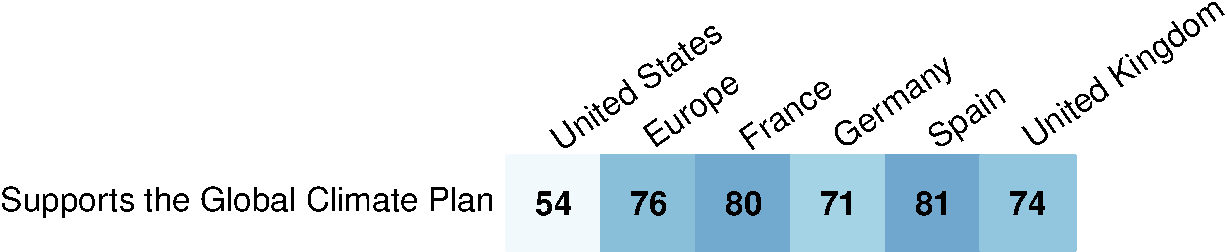
\includegraphics[width=1\textwidth]
  {../figures/EN/gcs_support_positive.pdf}}\label{fig:gcs_support} 
\end{figure}

\subsection{Genuine support} %

Despite the very favorable responses to the Plan, one might question the declared support. 
The only way to be absolutely certain that a majority of the population sincerely supports the Plan would be to organize a referendum. That said, even a simple survey can give a good indication of the sincerity of responses, and we used a number of methods to test this sincerity in the remainder of the survey.

To get as close as possible to the stakes involved in a referendum, we asked respondents whether they would be prepared to sign a petition in support of the Global Climate Plan, in the knowledge that the results of this question (asked of a representative sample of the population) would be forwarded to the Head of State's office. In this way, respondents understood that their response could influence official policy. In the USA, a majority were prepared to sign the petition, and the difference with direct declared support was not significant. In Europe, 69~% of respondents would be prepared to sign the petition~: this is 7 points less than for declared support, but still a large majority. 

Using a technique called <<~list experiment~>>, we show that support is genuine and not driven by a possible social desirability bias. This experiment works as follows~: we ask respondents \textit{how many} measures they support from a list of measures, and so we don't know whether a respondent supports this or that measure\footnote{As a result, respondents no longer face a social desirability bias prompting them to lie about their support for this or that measure.}. 
For a random half of the respondents, we add the Global Climate Plan to the list of measuresfootnote{In Europe, the three other measures on the lists are~: the death penalty for major crimes, a national redistribution plan and a building insulation plan}. 
By calculating the difference between the average number of measures supported in the groups with and without the Plan in their list, we can estimate the tacit support for the Plan. For example, if the \textit{group without} the Plan supports an average of 2.1 measures, and the \textit{group with} the Plan supports 2.86 measures, we can assume that the \textit{group with} the Plan supports the other measures as much as the \textit{group without} (since they are each representative of the population), and that the difference between the number of measures supported corresponds to support for the Plan, i.e. $2.86 - 2.1 = 76~\%$ tacit support for the Global Climate Plan.}. %
Tacit support is not significantly different from declared support, indicating that respondents are not pretending %.
support the Plan to meet a social standard%.
\footnote{In other contexts, this method has revealed a social desirability bias in favor of the invasion of Ukraine among the Russian population (tacit support being 10 to 20 points lower than declared support), or the under-reporting of racist opinions in the American South \citep{kuklinski_racial_1997,chapkovski_solid_2022}.}. 

\subsection{An electoral gain from campaigning for the Plan}
The most convincing proof that support for the Plan runs deep is that a progressive candidate could win votes by supporting it. We show this through a number of questions. First, we describe a progressive and a conservative program corresponding to the typical programs of the main parties in the country. We present the choice between the two programs as that between the two candidates in the next major election (in France, the second round of the next presidential election), and then ask respondents which candidate they would vote for}. For a random half of the sample, we add the Global Climate Plan to the progressive program. In France, the progressive candidate would gain 11 vote points by including the Plan in his or her program. In the USA, the progressive candidate could gain 3 points, while in the other countries, the effect is not significantly different from zero. The electoral gain is highly significant in France (the $p$ value is 0.5~\%). For the USA, the $p$ value is 13~\%, i.e. not statistically significant at the usual 5~\% threshold, but with only a 13~\% chance that the progressive candidate would have no electoral gain by supporting the Plan. For the other countries, the electoral gain is not significantly different from zero (even at the 20~\% threshold).}. 
Thus, support for the Global Climate Plan would not cost a progressive candidate votes in any country, and could yield a significant electoral gain in France. 

In the next question, we draw two political platforms from a set of (rather progressive) measures, then add the Plan to one of the platforms. In Europe, respondents are asked to imagine that a left- or center-left coalition will win the next election, and are asked on which platform they would prefer this coalition to have been elected. In the USA, the question is framed as a hypothetical duel in a Democratic primary and asked only of non-Republicans (i.e. Democrats, independents and non-affiliates)}. The program containing the Plan is systematically preferred by a majority (ranging from 58~\% in the USA and UK to 64~\% in Spain, cf. Figure \ref{fig:conjoint_left_ag_b}). This question and the previous one reveal that support for the Global Climate Plan is not only sincere, but is also important enough to determine the electoral choice of some voters.
This interest in 
the global redistribution is confirmed in a question asking respondents to allocate 100 points to express their support for a set of measures (the same as above), with the instruction to award more points to the measures they support most. The Global Climate Plan is given higher than average priority, and is one of the most popular climate policies. Conversely, a climate measure enacted in the EU and California (the phase-out of new internal combustion cars) is one of the three least prioritized measures in each country. More generally, this question shows that global redistribution measures are a fairly high priority for the electorate, just behind the most popular measures~: raising the minimum wage and improving public services through additional funding for education and healthcare}. 

\begin{figure}[h!] 
  \caption[Influence of Plan on preferred program]{Influence of Plan on preferred program~:\ Preference for random program A containing the Global Climate Plan over program B not containing it (in %). (In the U.S., question asked only of non-Republicans).}label{fig:conjoint_left_ag_b}
  \makebox[\textwidth][c]{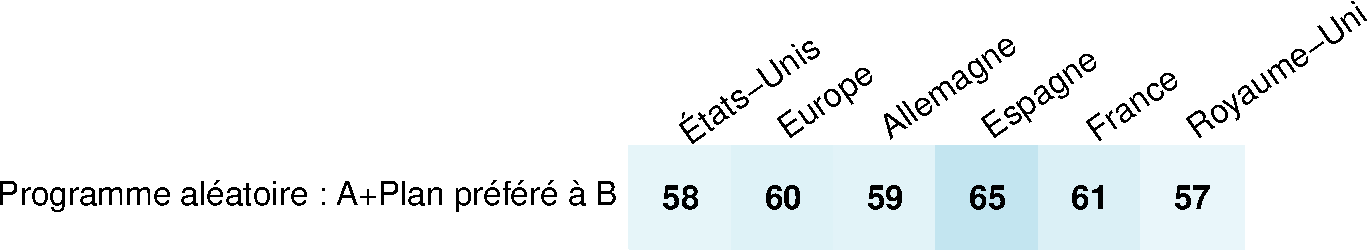
\includegraphics[width=textwidth]{../figures/FR/conjoint_left_ag_b_binary_positive.pdf}} 
\end{figure}


To sum up, the opinion polls reveal broad and sincere majority support for the Global Climate Plan, and indicate that the population prefers political programs that include this measure to those that do not. And this despite the fact that Western respondents are fully aware that they would lose some purchasing power under the Global Climate Plan. 

If people support this plan, it's because it's fair and global, and therefore effective in putting an end to climate change. This was not the case with the French carbon tax, which the Gilets jaunes opposed, and whose rejection was clearly measured in opinion polls. In other words, most people are concerned about the climate, and willing to support a solution as long as it is fair and effective. 
Find out more about these surveys%.
I refer the reader to the academic article entitled \textit{International Attitudes Toward Global Policies}, which I co-authored with Thomas Douenne and Linus Mattauch. 

\chapter*{\textit{Unfolding the political future dream}}\label{ch:narr_reve}
\addcontentsline{toc}{chapter}{nameref{ch:narr_reve}} 

The year I was born, the first conference on climate change was held. It was 1992, and economists were already dreaming up what would later become the Global Climate Plan. This idea was swept aside by the United States during the negotiation of the Kyoto Protocol, but received renewed interest when a study financed by the OECD revealed in 2023 that almost 80~\% of the population would support this Plan in all countries. This marked the start of a marathon of advocacy, first with economists, who were easy to convince, then with associations, who were less responsive, 
and finally to the political world. At the time of writing, the Plan has already received the blessing of several Nobel Prize winners, and we have presented it to the Chinese, Indian, Brazilian, French, German, Spanish and South African governments, all of whom have been receptive, %.
and was officially endorsed by seventeen European election lists from nine different countries (including Ecologistes -- EELV, Parti Socialiste and Renaissance -- Besoin d'Europe in France, and Sumar in Spain). 
This is the history we can write together, to put an end to climate change and extreme poverty. 

~[\textit{Beginning of fiction}] The Brazilian presidency of COP 30 put forward the idea ahead of the 2025 summit. It was immediately supported by Greta Thunberg and UN Secretary-General Antonio Guterres. 
Behind the scenes, the Chinese Foreign Minister is discussing the Plan with his European counterpart.  
Even if the negotiations remain secret, the German Social Democrats and Greens have decided to campaign on this Plan in the 2025 elections. 
Against all the odds, their coalition won by a landslide. 
All hell breaks loose. In November 2025, Brazil, the European Union, China and India make this plan their common position at COP29. Following Donald Trump's re-election, the United States obviously rejects the agreement, but the governors of California and New York state make it known that their states will join the agreement, even if the federal level does not follow suit. African countries can't believe their eyes~: 
are we really going to get an international agreement %?
on a plan that would double the average income of a country like Burundi, by paying every human a basic income of 40~euro{}/month~? In February 2026, a group of 156 countries and 9 US states, covering 74~\% of global CO$_\text{2}$ emissions, signed an agreement in principle to negotiate a cap on their CO$_\text{2}$ emissions. What followed was a five-year battle to negotiate the plan, followed by a painstaking implementation, which would be delayed but fully operational by 2037. Boosted by the basic income, Africa experienced an unprecedented economic boom. In the 2050s, the USA and Russia finally join the Climate Union. Saudi Arabia was the last country to take the plunge, in 2061. By 2084, the entire world has achieved carbon neutrality, and no one lives on less than $8 a day. Half of humanity is living below this poverty line at the time of writing. %
And you, strikers --- I'm sure you're part of it, you've got a lot to do with it. Indeed, none of this would have been possible without the global strike for justice and climate in October 2025, followed by almost a billion people.

\chapter{The main elements of the World Climate Plan}}

The proposal developed in this chapter does not solve all humanity's problems, nor is it a complete answer to climate change. Although it is referred to as <<~Global Climate Plan~>> (because it's more punchy), <<~International Fossil Energy Exit Framework~>> would have been more accurate.  %
As it stands, the Plan only covers fossil and industrial CO$_\text{2}$ emissions, not those linked to land use, forestry or other greenhouse gases. %
Its scope is limited to establishing a framework treaty that guarantees emissions reductions and determines international transfers. It is then up to each State or local authority to take the appropriate measures (climatic and social) to ensure that decarbonization proceeds smoothly on its territory. Now that the scope of the treaty has been defined, % of
Let's take a look at the Plan's main principles.

\section{1$^\text{er}$ principle~: An annual emissions quota}label{sec:pcp_quota}

The carbon budget --- and with it the future climate --- is the decisive element that the States will have to negotiate. 
Our proposal is based on a net emissions budget and covers the period when net emissions are positive, i.e. when emissions exceed sequestration (see below). Figure \ref{fig:emissions_par_region} illustrates a global emissions trajectory on which countries could agree, and projects the trajectories it might imply in different regions (see details in Appendix \ref{app:country}). 

\begin{figure}[h!]
  \caption[Emissions trajectories by region]{Estimated trajectories of CO$_\text{2}$ emissions per adult in different regions for a +1.8\textdegree{}C scenario}{fig:emissions_par_region}
  \makebox[\textwidth][c]{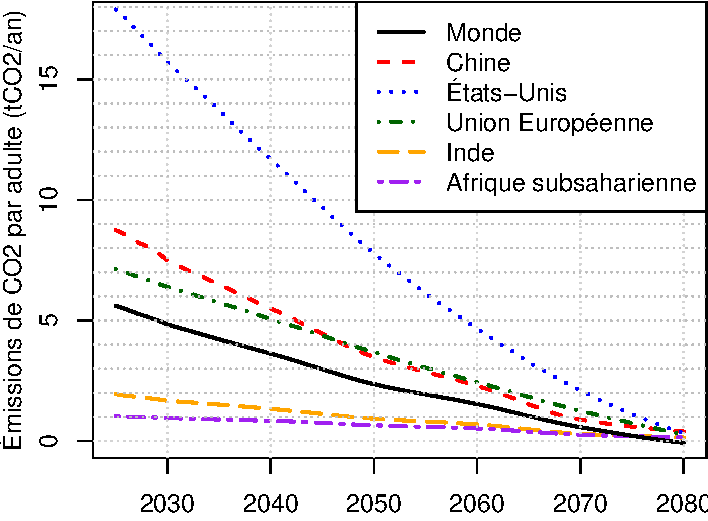
\includegraphics[width=.92\textwidth]{../figures/policies/emissions_par_region_sm.pdf}} %
\end{figure}

%%%%%% INSERT TODO %%%%%%%%%%



\section*{normalsize Is it possible to ensure a decent life for everyone in a decarbonized world~?}\label{q:decent}
\addcontentsline{toc}{section}{nameref{q:decent}}

Yes, the problem is not technical, but political. There are numerous scenarios showing how we can transform our society to achieve climate neutrality worldwide. The IPCC publishes scenarios compatible with warming limited to 1.5°C, others to 2°C, and so on. The most ambitious scenarios in terms of climate and poverty reduction call for a major reduction in consumption in high-income countries, through both efficiency gains and sobriety. \cite{oneill_good_2018,hickel_is_2019} show that a decent life could be ensured for 7 billion human beings while respecting planetary limits, provided there is a decrease in consumption in high-income countries. \cite{millward-hopkins_providing_2020} calculate that a decent life could be assured for all humans in 2050 while reducing energy consumption to its 1960s level, despite a population three times larger (this would require a 60~\% reduction in energy consumption per human). While it's clear that sobriety would make it much easier to achieve ecological goals, some scenarios detail how warming could be limited to 1.5ºC with <<~green growth~>>. For example, the \cite{agence_internationale_de_lenergie_net_2023} presents a scenario where the planet would achieve climate neutrality by 2050, while doubling global GDP by that time. 

Detailed models show the transformation required to decarbonize each sector in each country. In these scenarios, the bulk of decarbonization is based on technologies already deployed on a large scale (renewable energies, batteries, building insulation, heat pumps) or in the process of being deployed (green hydrogen, low-carbon steel and cement, carbon capture). In other words, technologies can be deployed to do without fossil fuels and to remove the CO$_\text{2}$ from the atmosphere due to residual emissions. Without these technologies, we would have no way of halting climate change, since reducing emissions is not enough --- we need to bring them down to zero. 

However, it is unlikely that technologies will be deployed quickly enough to limit warming to 1.5°C. Policies and actions 
current trends point to a warming of 2.6\textdegree{}C to 2.9\textdegree{}C by 2100footnote{Cf. \href{https://climateactiontracker.org/global/temperatures/}{climateactiontracker.org/global/temperatures}.} and a temperature that will continue to rise at an alarming rate after 2100. In this context, the greater the efforts to reduce consumption, the more warming will be slowed down. 

These observations should bring the proponents of degrowth into line with those of green growth. On the one hand, we need to stimulate growth in \textit{productivity}, in particular to improve our energy efficiency and deploy greener technologies. On the other hand, we need to encourage a decline in \textit{overconsumption}, to reduce the damage that exceeding planetary limits inflicts on the most vulnerable. 

\section*{normalsize Who pays in the proposed system~: companies or consumers~?}label{q:incidence}
\addcontentsline{toc}{section}{nameref{q:incidence}}

In economics, we need to distinguish between legal and economic impacts. Legally, it is the companies upstream of the production chain that would be subject and would be obliged to buy emissions permits. But this legal impact does not make it clear who will pay. In principle, the companies subject to the measure could react in one of three ways~: by reducing their profits, cutting their wages, or raising their prices. The cost of the measure would then be passed on respectively to shareholders, workers in polluting sectors, or consumers. \cite{ganapati_energy_2020} estimates that around 70~\% of the energy price rises faced by the manufacturing sector are passed on to consumers in the short to medium term, with the remainder absorbed by shareholders. In the long term, we can expect the rate of profit to stabilize, and consumers to pay the full cost. This is the mechanism described in Chapter 2: the price of carbon is paid by consumers, in proportion to their carbon footprint. In fact, that's the whole point of carbon pricing~: unless the price of carbon-intensive goods rises relative to low-carbon options, there would be no incentive to reduce emissions.

\section*{normalsize What about other greenhouse gases~? Other planetary limits~? Biodiversity~?
\addcontentsline{toc}{section}{nameref{q:scope}}

Alas, the proposed Plan does not address these issues. It is therefore necessary to consult other works in order to put together a program that would respond to all the ecological challenges{for example \citet{strassburg_reducing_2009,karsenty_geopolitique_2021} in the case of forests}. %
Let's just note that the Plan's logic could be replicated to solve other problems (not all of them). For example, we could imagine an equivalent quota system for exhaustible resources such as metals or fish stocks. Extraction permits %
or fishing would be auctioned off, and the proceeds distributed equally among all humans.

\section*{normalsize Won't emissions rise if we double the incomes of the poorest~?}\label{q:emissions}
\addcontentsline{toc}{section}{nameref{q:emissions}}

If we were simply to redistribute income, emissions would rise, since the poorest people devote a greater proportion of their income to the consumption of carbon-intensive goods than the wealthiest. Even so, the increase would be fairly limited. \cite{sager_income_2019} estimates that a complete equalization of American incomes (at constant average income) would increase their greenhouse gas emissions by 2~\%. Similarly, \cite{oswald_global_2021} find that with near-complete equalization of human incomes (reducing the maximum income to twice the minimum), energy consumption would increase by 7~\%. 
But, by construction, the Global Climate Plan would cap emissions on a downward trajectory. As a result, emissions could only fall. The spectacular rise in consumption (and therefore emissions) by the poorest would be more than offset by the fall in consumption by the richest, and by decarbonization (i.e. the reduction in emissions linked to a given level of consumption).

\section*{\normalsize Doesn't this system benefit the richest, by allowing them to buy a right to pollute~?}\label{q:riches}
\addcontentsline{toc}{section}{nameref{q:riches}}

A recurring argument against carbon pricing is that it would give the richest a free pass to pollute, and shift the cost of decarbonization onto the middle classes, who can't afford the price rises. 

The short answer to this objection is that we need to be clear about what we're comparing ourselves to. If we compare the Global Climate Plan with a far more radical proposal, such as a way out of capitalism where incomes would be capped at 3~000~\euro{} per month, then the richest people are indeed doing well. On the other hand, compared to the status quo, the richest lose out, and all the more so when the complementary measures described in Chapter 1 are implemented. 

For the long answer, let's start by recalling the Plan~'s distributional effects: individuals with a high carbon footprint would lose out financially, while individuals with a carbon footprint around the world average could make the ecological switch without losing purchasing power. These <<~average~>> individuals would be incentivized to change their equipment and habits by the carbon price, and those who switched to decarbonized options faster than others would become financial winners (since their carbon footprint would fall below the global average). On the other hand, the middle classes in high-income countries have a carbon footprint higher than the world average~: they would therefore lose out financially if they did not adapt, and adaptation itself presents a cost (monetary or comfort) in any case. However, the better-off would lose even more, since they have an even higher carbon footprint. 

Of course, it's fair to say that the better-off have more leeway to adapt, and should be asked to contribute even more than the Plan implies. It is for this reason that I advocate additional measures of national redistribution (cf. Chapter \ref{ch:premier_pas}) to ensure that the full cost of decarbonization is borne by the most affluent, and to preserve the standard of living of the middle classes in high-income countries. However, if the majority of the population supports national redistribution measures, it's because they consider the distribution of wealth too unequal, whether there is a climate policy or not. In other words, we can separate the two proposals~: on the one hand, a climate policy that does not aggravate inequalities (in fact, the Global Plan reduces them)~; on the other, a national redistribution policy that puts an end to an indecent level of inequality. If we were looking for a complete political program, we'd have to include these two proposals, as well as many others. But that's not the purpose of this book. We focus here on one proposal, and design it in such a way that it can be supported by individuals and governments of all stripes. 

To sum up, I believe that the Global Climate Plan is preferable to the status quo, and should be complemented by additional redistributive measures. In the following questions, I will explain why I believe it is preferable to alternative climate measures. 


\section*{\normalsize Wouldn't this Plan allow capitalism to continue, when it should be overthrown~?
\addcontentsline{toc}{section}{nameref{q:capitalism}}

So as not to enter into an endless debate between reformism and revolution, I'll confine myself to three arguments. Firstly, we can support the Global Climate Plan as a step in the right direction, while preferring and developing a more ambitious plan. Secondly, the extent of the redistribution brought about by the proposals in this book seems to me to be close to that which one would expect to be the most radical %.
in the coming decade, given the current balance of power --- dominated by affluent social groups who value their level of comfort. %
Thirdly, even in a post-capitalist society, emissions would have to be capped in a binding way, and the proposed Plan seems to me the best option for doing this (as explained below). 

\section*{\normalsize Shouldn't we just %.
prohibit activities destined to disappear and subsidize those destined to develop~?}label{q:interdiction}
\addcontentsline{toc}{section}{nameref{q:interdiction}}

There are certainly standards to be introduced, activities or products to be banned and others to be subsidized. For example, we could ban the sale of combustion-powered vehicles and gas or oil-fired boilers, as well as the construction of steelworks, cement works and power plants that exceed a certain level of emissions. Subsidies could make the cost of decarbonized equipment bearable for households, and new low-carbon plants competitive with existing polluting plants. For decarbonization to take place in this way in the countries of the South, the countries of the North would undoubtedly have to finance their subsidies, but this is also conceivable. There's nothing to stop such measures being put in place as a complement to the Global Plan --- and that's what the proposals in Chapter 1 are all about. If these bans and subsidies were to reduce emissions below the agreed ceiling, the price of carbon would be zero, as there would be no need to incentivize further emissions reductions. The Global Climate Plan would then be painless. But it would be no less useful. Indeed, it is not certain that bans and subsidies will generate sufficient emissions reductions~: the cap introduced by the Plan offers a valuable guarantee in this respect.

In addition, standards, bans and subsidies have a number of shortcomings that make them unsuitable for certain situations. Firstly, they don't always benefit the most modest~: for example, subsidies for thermal renovation can disproportionately benefit homeowners (whose homes will increase in value following renovation), while bans on polluting vehicles in city centers affect more modest households. Secondly, standards and subsidies often create a rebound effect, reducing their effectiveness by driving up consumption. For example, subsidizing electric cars encourages car use rather than cycling or public transport. 
Economically, a bonus/malus on the purchase of an electric/polluting vehicle is equivalent to a standard on the emissions (of the average) of new vehicles, and these measures both lead to greater use of the car compared to carbon pricing. And if we subsidize all means of transport so as not to favor the car, we are unnecessarily encouraging mobility, and with it urban sprawl and journey times. %
Thirdly, sector- or technology-specific regulations are less efficient than indiscriminate emissions pricing, as they discretionarily favor specific sectors or technologies. This effect is not even related to the fact that specific regulations may be more prone to lobbying, corruption or administrative errors. 
To understand, let's imagine that a country favors renewable electricity through subsidies or binding targets, rather than pricing CO$_\text{2}$ emissions from the power sector. This is broadly what the United States has done. Coal is thus not penalized in relation to gas (which is less polluting), and its use in electricity generation is therefore excessive. %

These shortcomings need to be set against the shortcomings of carbon pricing, and in particular the disparities in situations it creates, see Section \ref{sec:mue_nationale}. In the absence of a miracle solution, the optimum solution is to implement a panoply of complementary measures, in which pricing as well as standards, bans and subsidies have their place. The Global Plan has a place in this panoply because it offers two major advantages~: firstly, it makes it possible to define and guarantee an international climate ambition, in the form of a carbon budget~; secondly, this Plan is easier to negotiate than alternative agreements. Indeed, the main element of the Plan to be negotiated is the carbon budget. Alternative agreements are conceivable, for example transfers from Northern countries in exchange for climate action by Southern countries. South Africa, Indonesia, Senegal and Vietnam have each signed a Just Energy Transition Partnership (or JETP) with a group of Northern countries. Indonesia, for example, has pledged to accelerate its phase-out of coal and the decarbonization of its electricity system in exchange for \$20 billion in financing, mainly in the form of concessional loans \citep{ha-duong_just_2023}. A group of Northern countries have pledged to provide this financing, subject to the fulfillment of this commitment. Compared to the Global Climate Plan, JETPs suffer from several shortcomings~: they finance middle-income countries, do not tackle poverty, and involve relatively low transfers from Northern countries. In reality, JETPs enable banks in Northern countries to finance profitable projects in Southern countries. What's more, the coverage of JETPs is far from systemic, since they concern only a few countries in the South, and are unlikely to extend beyond the power sector. In short, JETPs cannot guarantee compliance with the carbon budget or put an end to extreme poverty}. 
(such as a credible plan to decarbonize a growing electricity sector). If countries manage to negotiate an agreement that determines a decarbonization trajectory as ambitious as the Plan's, with equivalent North-South transfers (around 1~\% of global GDP), then this agreement could well replace the Plan. In the meantime, it seems to me easier to agree on the Plan than on a set of measures differentiated by region and sector.


\section*{\normalsize Why a carbon market rather than a tax~?}\label{q:tax}
\addcontentsline{toc}{section}{nameref{q:taxe}}

The advantage of a carbon market is that it places a cap on emissions, ensuring that the desired emissions trajectory is followed. If the trajectory of the tax is set in advance, there's a good chance that the level required to achieve the climate target will be wrong, and that the tax will be set either too low or too high. If the level of the tax is automatically re-evaluated each year so as to keep emissions on the desired trajectory, we end up with a system rather like the carbon market. The difference between the two is one of detail~: the market adjusts immediately to new situations (such as war or the entry of a new country into the system), at the cost of an ecosystem of financial players who analyze, operate and earn a return on this market. As the two systems are very similar, an automatically reassessed tax would be just as appropriate. However, I prefer to present the Plan in the form of a market, so as not to be confused with the usual carbon taxes, whose trajectory is fixed in advance. 

Finally, if the level of the tax were re-evaluated each year by a political decision (rather than automatically), this would offer interest groups endless opportunities to question the level of climate ambition and deviate from the climate target. To better resist such pressures, it seems to me preferable to set the emissions trajectory in advance. This preference means prioritizing the climate objective, even if it means accepting major reductions in living standards if decarbonization proves more costly than expected. 
On the contrary, some would probably prefer to limit efforts in the short term, even if it means inflicting more damage on future generations if efforts prove less effective than expected. If this latter inclination were in the majority, the climate objective could no longer be guaranteed. We would then have to resolve to have a ceiling price on the carbon market, or a carbon tax whose level would be chosen politically, as proposed by \cite{weitzman_world_2017}. 

\section*{\normalsize Why not a progressive carbon tax~?}\label{q:taxe_progressive}
\addcontentsline{toc}{section}{nameref{q:taxe_progressive}}

Some authors, such as Thomas \cite{piketty_capital_2019}, advocate a progressive carbon tax, with the first few tonnes of individual emissions taxed little or not at all, the next tonnes taxed more, and so on up to a maximum level of emissions. In my opinion, this is a false good idea. 

First of all, we are far from having the administrative means to accurately calculate an individual's carbon footprint~: to do so, we'd need an international treaty obliging companies to declare their transactions. Admittedly, such a treaty would be welcome, and even without it, carbon footprints could be approximated. But approximating carbon footprints would reduce incentives to decarbonize. For example, by attributing the same carbon content to each smartphone, a smartphone manufacturer would have no incentive to make any effort, since it would not be distinguished from the others. Both administratively and economically, it is more efficient to make the producer upstream in the value chain pay the price, rather than the consumer downstream. 

But the real pitfall lies elsewhere~: the effects of such a measure would not necessarily be desirable. Let's take two individuals with an income of 2~000~euro{} a month~: one lives in a poorly insulated bungalow, heated by oil, and drives 50 km a day to work~; the other lives in a well insulated building, heated by geothermal energy, and gets around by bike. The former has a carbon footprint five times higher than the latter. With conventional carbon pricing, the former already loses purchasing power to the latter. With taxation that increases with carbon footprint, the disparity widens even further. On the contrary, we should probably seek to reduce the disparities in the effects of climate policies between these two types of people (this is the sense of the complementary measures proposed in Chapter 2). Ultimately, such a proposal would be interesting if the carbon footprint at which the tax rate increases were high enough to spare the middle classes (say, at 30 tonnes of CO$_\text{2}$ per year), or if it only applied to aviation. %

But progressive carbon taxation could take a more relevant form~: the tax rate could rise with the individual's \textit{income}, rather than with his \textit{carbon footprint}. This would avoid exacerbating disparities in effects for the same level of income, while disproportionately penalizing the richest. Such a solution would make it possible to impose a comparable level of decarbonization effort on all income levels. 

These two forms of progressive taxation would come up against a common problem~: the case of companies. At what rate should a company's emissions be taxed~? If taxed at a low rate, the more affluent will have an incentive to pass off their personal expenses as business expenses. Taxing them at a high rate, on the other hand, would encourage informal work, as well as fraud in the other direction, where employees would pass off business expenses as personal expenses (in exchange for bonuses). It would therefore probably be necessary to tax corporate emissions at an intermediate rate. To avoid fraud, a small gap could be chosen between the minimum and maximum rates, but this would reduce the scope of the measure. Another option would be to allocate certain company expenses (travel, catering, accommodation) to the individuals who benefit from them (generally employees), and to tax these individuals, at least above a certain expenditure threshold. 

Ultimately, if the aim of such proposals is to reduce inequalities, it seems simpler to me to complement the Plan with a redistribution of wealth, as proposed in Chapter 2. That said, the last suggestion is worth exploring. It is not incompatible with the Global Climate Plan~: the latter could be supplemented by additional taxation of the carbon footprint of the wealthiest. 

\section*{\normalsize Why not ration individual carbon footprints~?}\label{q:rationing}
\addcontentsline{toc}{section}{nameref{q:rationing}}

Some percentages
peoplefootnote{wood_rationing_2023}.} propose a system of rationing individual emissions, where emissions trading would be prohibited. In other words, unlike our Plan, which reverts to a system of tradable carbon quotas, rationing would prohibit individuals from buying permits if they have a shortage, or selling them if they have an excess. %
Rationing would be problematic for several reasons. 

Already, if emissions permits were not tradable, this would mean either that hundreds of millions of people (particularly in northern countries) would have to halve or treble their emissions overnight, making it impossible for them to continue their daily activities~; or that more emissions permits would be allocated (initially) to those who pollute more, breaking with the principle of equality dear to the advocates of non-tradable quotas. Conversely, if permits were tradable, polluters would have some latitude regarding their emissions, and time to gradually adapt their activities and change their equipment. As for people with a low carbon footprint, they could resell their unused emissions permits and thus gain purchasing power. In this way, both polluters and the frugal would benefit from the flexibility enabled by the market. In fact, the potential benefit would be so great that the emergence of a black market would be difficult to prevent in the case of a non-tradable quota system. 

\section*{\normalsize Is it moral to let the rich buy rights to pollute~?}\label{q:moral}
\addcontentsline{toc}{section}{nameref{q:moral}}

You may be thinking that a carbon market would be immoral or unfair, as it would allow the richest to continue polluting. However, such a system would redistribute resources from polluters to the frugal~: the latter would have to pay to buy emission permits from the former. What's more, setting up a carbon market wouldn't prevent us from banning consumption deemed superfluous, such as yachts, private jets and even SUVs. Finally, if we consider it unfair that the wealthiest are able to maintain an expensive lifestyle in such a system, isn't it because we consider extreme wealth to be unfair~? If that's the case, we might as well attack wealth directly, rather than through the back door. Indeed, capping Rupert Murdoch's emissions wouldn't have prevented him from using his media empire to minimize or even deny climate change. Moreover, capping billionaires' emissions wouldn't even prevent them from using a private jet~: they'd simply replace kerosene with agrofuels or hydrogen. If the aim of rationing is to prevent lavish activities, %
If we wish to limit (rather than ban) a particular activity such as flying, we could ration this activity. However, even from this point of view, where we are not satisfied with the price of carbon, it seems preferable to devise a system of differentiated authorization (or even taxation) to distinguish justified flights (business or family reasons) from superfluous flights (tourism). 
} of these activities or a cap on wealth.  %

\section*{\normalsize Is a basic income the best way to distribute resources to the poorest~?}\label{q:rdb}
\addcontentsline{toc}{section}{nameref{q:rdb}}

Basic income offers several advantages. Firstly, if properly implemented, it can reach all human beings, leaving no one by the wayside. Conversely, if funds were allocated to institutions rather than individuals, certain social groups (such as urban dwellers, men, or groups in power) could be favored to the detriment of others. On the other hand, a basic income meets the needs of each individual and empowers everyone. Finally, scientific studies show that unconditional cash transfers in low-income countries bring significant improvements in nutrition, well-being and health, as well as an increase in activity (with many taking advantage of the basic income to invest in their micro-businesses) and lasting enrichment. Compared with targeted transfers (to certain countries or to the most disadvantaged) or conditional transfers (e.g. children's attendance at school), a basic income has the immense advantage of simplicity and universality, making its distribution less prone to error, abuse and criticism. The main disadvantage of the basic income is that its distribution requires an infrastructure that has yet to be built in some countries (see Section \ref{sec:implementation}).  %

The alternatives have their advantages too. Distributing resources to the government enables the development of public services and social protection. Allocating the money to local authorities (communes, village chiefs, citizens' associations, economic interest groups) makes it possible to finance collective works (sanitation, irrigation, etc.). In addition, the development of countries in the South also requires the financing of large-scale projects (dams, railway networks, etc.) managed by the State or development agencies. 

If these institutions are worthy of funding, their financing can be based on 
basic income rather than replacing it. In fact, by increasing the population's income and developing a means-of-payment infrastructure, the basic income will enable local and national authorities to levy more taxes. Also, rather than deducting the same amount from every human being (which would be the case if all or part of the basic income were paid directly to the authorities), these taxes could be progressive, i.e. concentrated on the wealthiest. 

For these reasons, a basic income is the most desirable option. That said, as explained in the Plan's timetable (Appendix \ref{ch:details}), the form the payment will take must be chosen by the local population. If the basic income proves unsuitable in certain contexts, or if the infrastructure for its distribution is not yet ready in some places, an alternative could be preferred, respecting the principle of allocating revenues proportionally to the local population. 

\section*{normalsize Can fraud be avoided~?}\label{q:fraud}
\addcontentsline{toc}{section}{nameref{q:fraude}}

A well-designed system would largely prevent fraud. Section \ref{sec:implementation} shows that it is possible to check that emissions are correctly reported thanks to satellite observations, and to guarantee that no-one receives the basic income more than once thanks to biometric identification. What's more, a country that fails to implement carbon pricing or pay the basic income correctly on its territory would face sanctions up to and including exclusion from the climate union. 

Another type of fraud occurred when the European carbon market was launched in 2009~: VAT fraud on carbon allowances. This fraud was made possible by a design flaw in the system for making allowances subject to VAT, which was corrected in 2010. Such fraud has not been repeated on other carbon markets, since the authorities are now vigilant about their design.


\section*{normalsize Won't the public oppose the Plan when they realize the magnitude of the effort required~?
\addcontentsline{toc}{section}{nameref{q:soutien}}

Even if it's impossible to predict the future, it seems unlikely that the public will oppose the Plan, and even less likely %.
that it is more opposed to the Plan than to a national climate policy of equivalent ambition, for several reasons. 

On the one hand, representative surveys accurately reflect %.
public opinion. 
For example, during the Gilets jaunes movement, 
only 13% of French people said they supported the carbon tax. Note that a few months before and a few months after, support was at a much higher level. A new survey showed 38% support for the same measure two years after the beginning of the movement. While these surveys reveal that opinion on a climate policy can change substantially with the context, the variation in support from one year to the next remained contained at less than 25 points. Similarly, the effect of a negative media campaign on the Plan was estimated at 11 points less support 
in the United States. Even if support for the Plan were to fall by 25 points, it would still be in the majority in Europe, since it currently stands at 76% (see Chapter \ref{ch:support}). Admittedly, with a change in opinion, support could become a minority in the USA, but we are already working on the assumption that the USA will probably not participate in the Plan. 

Furthermore, the surveys converge on a number of aspects consistent with strong support for the Plan. Firstly, the surveys all show that most people are concerned about climate change and support climate action. For example, representative surveys in 125 countries show that 89~\% of the world's population believe their national government should do more to combat climate change, and 69~\% say they are willing to contribute 1~\% of their income to do so. %
Secondly, surveys have shown that two-thirds of Americans and eight out of ten French people are <<~ready to adopt a green lifestyle (i.e. eat little red meat and make sure they use almost no petrol, diesel or
kerosene)~>>, <<~assuming that all the world's states were to agree to take firm action against climate change, in particular by making a
transition to renewable energies, by putting the richest to contribution, and by imagining that [the country] very largely extends the offer of non-polluting transport~>>footnote{In France, there are 65~\% of \textit{Yes} vs. 17~\% of \textit{No} \citep{douenne_french_2020}~; in the United States, it's 51~\% vs. 26~\% (unpublished results from \citealp{dechezlepretre_fighting_2022}), the rest are undecided}. %
Thus, a large majority of human beings declare themselves ready for ecological change, even when the monetary cost or change in lifestyle required is made explicit. 

If these statements seem disconnected from everyday choices, it's mainly because individual efforts are conditional on a systemic shift. In addition to aspirations to justice and material needs, this conditionality is also linked to the tendency of individuals to conform to the norm of their social group. Research in social psychology has shown that individuals have ambivalent attitudes, linked to aspirations that conflict with one another, and that, depending on the context, one facet of their identity is activated rather than another. %
If, at present, the social context favors the activation of a consumerist and individualist identity, the balance could quickly change, as many people are ready to activate another mode of their personality, more frugal and altruistic.

Finally, studies on the subject have highlighted three key perceptions for public support for a climate policy~: whether the measure is (perceived as) effective in combating climate change, in the interests of the most modest, and in its own personal interest. The importance of effectiveness helps explain why climate policies on a global scale are preferred to decarbonization measures that are just as rapid, but confined to the national level~: only global action can put an end to climate change. The Global Climate Plan meets the first two criteria (effectiveness and social justice), and provided it is complemented by national redistribution (as proposed in Chapter 1), it will also protect the interests of the Western middle classes. By shifting the bulk of the cost of ecological change to the better-off, this solution has every chance of being supported by the majority of the population, even in high-income countries. Insofar as the Western middle classes would be no more affected by the proposed solution than by a national decarbonization program, they would have no reason to protest against the Global Plan. In view of this, it seems far less likely to me that a social movement will arise against the Global Plan than against a carbon tax that harms the middle classes (such as the one behind the Gilets jaunes) or against the ban on the production of combustion-powered cars (due in 2035 in the EU). Of course, there is a chance that the wealthiest will oppose the Plan, as they will be the big losers. The challenge will then be to ensure that the majority of the population prevails over the elite, as is supposed to happen in a democracy.


\section*{{normalsize In what currencies will the exchange of permits and the distribution of the basic income be carried out~?}\label{q:devise}}
\addcontentsline{toc}{section}{nameref{q:devise}}

During the auction, any national currency will be accepted to buy emission permits. The conversion rate used will be the market rate at the time of the deadline for the transmission of purchase options}. The basic income will be distributed in the national currency. The organization responsible for auctioning and paying out the basic income will enter into \textit{exchange swaps} with the central banks of various countries to acquire the necessary local currencies. In practice, the central banks of low-income countries will accumulate reserves of heavily-used currencies (dollar, euro, renminbi), which will improve the financial stability of these countries and enable them to finance imports.

\section*{{normalsize What will be the macroeconomic consequences of the Plan (growth, inflation, unemployment)~?}\label{q:macro}
\addcontentsline{toc}{section}{nameref{q:macro}}

As with any decarbonization policy, the Plan will boost activity in certain sectors (renewable energies, construction, mining) and reduce activity in others (fossil fuels, aviation). This will result in job creation outstripping job destruction in most countries, as well as the relocation of workplaces and housing. As a result, unemployment is set to fall overall, even if it will rise in some areas. The effect on global growth should be positive, although final household consumption will grow less rapidly than in the absence of ecological change. This is because a greater proportion of activity would be devoted to investment, the benefits of which (in terms of energy savings in particular) would only materialize after the fact. 

Although hydrocarbon-exporting countries will lose significant resources as a result of decarbonation, the countries most affected will be those in the Gulf. In particular, Iraq, Iran and Algeria combine an economy heavily dependent on fossil fuels with a GDP insufficient to overcome the loss of revenue from hydrocarbon sales \citep{muttitt_equity_2020}. 
Thanks to the "opt out" clause, which allows them to keep the carbon pricing revenues linked to the fossil fuels they place on the world market, %CO
these countries would recover a share of the revenues they would have totally lost in the event of unilateral decarbonization by the rest of the world.
}, we shouldn't overestimate the job losses it would generate worldwide. These are estimated at 28 million (against 52 million jobs created) by a studyfootnote{Cf. \cite{jacobson_100_2017}. According to the study, 22 countries are facing a net loss of jobs. The hardest-hit countries were Brunei (9~\% of jobs destroyed on net), Libya (7~\%), Qatar (6~\%), Norway (5~\%), Kuwait (5~\%), Saudi Arabia (3~\%) and Iraq (2~\%),} and 9 million (versus 14 million created) by another study.
\footnote{\cite{pai_meeting_2021}. More than the quantity of jobs, it's the quality and location of the jobs created that may pose a problem \citep{haywood_welfare_2021}.}. In other words, decarbonization would destroy at most 1~\% of global jobs and create twice as many. In terms of employment, the scale of the transition is therefore limited, compared with automation, which threatens 10 to 50~\% of jobs{footnote{cite{frey_future_2017,lassebie_what_2022,hatzius_global_2023}.}, or the mechanization of agriculture, which for example reduced the share of farmers in French employment from 36~\% to 10~\% between 1946 and 1976\footnote{Cf. \href{https://ourworldindata.org/grapher/urbanization-last-500-years?country=~FRA}{ourworldindata.org} and \href{https://ourworldindata.org/grapher/share-of-the-labor-force-employed-in-agriculture?tab=chart&time=1800..latest&country=FRA}{\cite{herrendorf_chapter_2014}}}.} and has caused urbanization to grow at the same rate. On the other hand, we shouldn't underestimate the lifestyle changes required by the ecological moult, and in particular the decline of the private car and beef consumption.

As with any global redistribution of wealth, the Plan will increase consumption and activity in the countries of the South, and decrease consumption by the wealthiest. Consumption of basic goods and services (food, infrastructure, healthcare, education) will increase, to the detriment of sectors such as luxury goods and tourism. While the economy adjusts, this redistribution will lead to higher prices for basic foodstuffs, and potentially lower prices in certain sectors (art, hotels, etc.).
). 
Note that initial inflation in low-income countries will necessarily be lower than the increase in purchasing power due to the basic income (inflation being caused precisely by the increase in purchasing power). 

Historical examples of massive inflows of development aid to Africa have shown that these transfers have positive effects in line with expectations (on inflation, trade, the exchange rate, interest rates and growth)}. As another example, Guyana has been able to absorb a doubling of its GDP between 2021 and 2022 (following the opening of an oil well) while keeping inflation under controlfootfootnote{\citet{fmi_guyana_2023}.}. 

The effect of such redistribution on the GDP of a country like France is ambiguous. On the one hand, increased growth in the South will boost exports of goods and services from the North (machine tools, engineering services, pharmaceuticals). 
On the other hand, the importance of declining sectors (luxury goods and tourism together account for 6~\% of French GDP%) is also a factor.
) would reduce national production. The total effect on GDP will probably not exceed one or two percent in either direction, and will in any case remain derisory compared to the benefits of the Plan (end of climate change and extreme poverty). 

Even if the macroeconomic mechanisms are well understood, and their quantification subject to the uncertainties inherent in modeling, such modeling is necessary to best anticipate the effects of the Plan. I intend to work on this with other academics in the near future.





\section*{{normalsize How does the Plan position itself in relation to other demands such as transfers for loss and damage or the fossil non-proliferation treaty~?}\label{q:climate_movt}
\addcontentsline{toc}{section}{nameref{q:climate_movt}}

Developing countries are demanding at least \$100 billion a year to compensate for the loss and damage to the climate caused by emissions from developed countries. This compensation stems from the historical responsibility of states, whereas the Global Climate Plan is concerned with future emissions. What's more, such financing would not be intended to cap CO$_\text{2}$ emissions, and would have no effect on decarbonization. %
So the Global Climate Plan is a parallel demand, not a substitute for loss and damage.

The Fossil Fuel Non-Proliferation Treaty is an international initiative for just decarbonization, spearheaded jointly by the climate movement, scientists and Pacific island countries. Contrary to what its name might suggest, no treaty has been drafted as part of this initiative, and its demands remain of a general nature. As a result, the Global Climate Plan is fully compatible with this initiative, and can even be understood as a possible instantiation of such a treaty.

\section*{\normalsize How would this system fit in with existing tools, such as the European carbon market~?
\addcontentsline{toc}{section}{nameref{q:ets}} %

To avoid slowing down the decarbonization of certain already ambitious countries, the Plan should be added to the instruments already in place. 

Let's take the example of the ETS, the European carbon market. Two cases are possible. The least likely case is that the European carbon price (just before the global system comes into force) is lower than the global price. Applying the global price would then be enough to bring European emissions back under the ETS cap, without the need for the European price mechanism~: the carbon price in the ETS would be zero. In the most likely case, the world price would be lower than the price needed in the ETS to bring European emissions within the European cap. In this case, the total carbon price (global + European) paid in the EU would not change when the global price is introduced, but the global price would absorb part of the European price. In other words, the EU would lose revenue to the rest of the world. Additional revenues would therefore be needed to perpetuate programs financed by ETS revenues, such as subsidies for thermal renovation. Once again, taxing the wealthiest could do the trick (see Table \ref{tab:redistr_policies}).











\appendix

\part*{Technical and methodological appendix}}label{appendix}
\addcontentsline{toc}{part}{nameref{annex}} 

\chapter{Plan details{label:details}} 

A number of points remain to be clarified for the Plan to be complete: its timetable, scope, framework, governance, market organization and participation mechanisms. 

\paragraph{Calendar} 
The Plan can be put on the agenda of the COPs and the G20, with a view to gradual implementation between 2030 and 2035. During the negotiation and preparation phase (before 2030), it is essential to ask citizens around the world if they would like to benefit from a basic income, and to study their potential concerns. Indeed, each community should have the right to opt out of the basic income (or to receive it in a different form, e.g. as a transfer to the whole community rather than to individuals), to avoid disrupting social structures. In addition, basic income schemes should start with very low amounts to ensure smooth implementation. Indeed, the redistribution effected by the basic income would lead to an increase in the demand (and price) of commodities. Despite inflation, the basic income would increase the purchasing power of low-income earners, but it's important not to leave anyone out, and to ensure that all those who want the basic income receive it. If the ETS is ready before the basic income, it could be implemented by (initially) allocating the revenues to the states.

\paragraph{Perimeter} 
A priori, the Plan would exclusively regulate CO$_\text{2}$\footnote{That said, on the model of the European carbon market, the Plan could also cover minor greenhouse gases, such as N$_\text{2}$O or PFCs.}. Although similar policies could be designed to regulate other substances, such as methane, it is more appropriate to deal with CO$_\text{2}$ separately in order to better manage its specificities. Ideally, the Plan should cover all CO$_\text{2}$ emissions, although it may be more practical to limit it initially to CO$_\text{2}$ from fossil fuels and cement production in large industrial units (i.e. a scope similar to the two European carbon markets combined). The Plan should also cover CO$_\text{2}$ emissions from international shipping and aviation. 

\paragraph{Frame} %
The international treaty establishing the Plan would have to specify certain non-amendable elements, including its perimeter, the use of its revenues, its governance rules and the carbon budget. The main element to be negotiated would be the carbon budget, and this should be defined in line with the Paris Agreement. A reference to the Paris Agreement would make it possible to define a carbon budget <<~Containing the rise in global average temperature well below 2°C compared with pre-industrial levels and continuing the action taken to limit the rise in temperature to 1.5°C~>>. One possible interpretation of this objective is to aim for a long-term temperature of +1.5°C, but to allow a temporary overshoot of up to +2°C. 
Considering that aiming for +1.5 GtCO$_\text{2}$\textdegree{}C means adopting a carbon budget that gives a 50/50 chance of reaching this target, this interpretation would define a carbon budget of 500 GtCO$_\text{2}$ from 2020 onwards, 
which would determine the Plan's carbon budget by subtracting emissions occurring between 2020 and the launch of the Plan. This budget would cover both the positive emissions budget for the first phase of the Plan and the positive and negative emissions budgets for the second phase (see Section \ref{sec:pcp_quota}). 
The complete % emissions trajectory
could then be chosen in line with the maximum overshoot target and up-to-date understanding of the climate system. 
In particular, the first-phase emissions budget to keep global warming below 2°C could be chosen with a probability of 67~\% (implying a budget of 1~150 GtCO$_\text{2}$ from 2020, or 1~000 Gt from 2024) or a probability of 83~\% (900 GtCO$_\text{2}$ from 2020). 

If certain countries do not participate in the Plan, the Plan's carbon budget will be adjusted downwards on the basis of equal emission rights for each human adult (in line with the principle of leaving the same emission rights to non-participating countries).

\paragraph{Governance} 
The Plan's governing body would define the annual emissions quota (in line with the Plan's framework), the market organization (\textit{market design}) and any sanctions against non-participating countries. %
The choice of sanctions would be the most political decision of the governing body. Sanctions could backfire on union members in the event of retaliation by sanctioned countries, and such retaliation would probably affect countries in proportion to their economic and geopolitical weight. 
Furthermore, the ETS would impose a cost on participating countries in proportion to their emissions. It therefore seems legitimate to grant each country a voting right proportional to its CO$_\text{2}$ emissions, as far as sanctions and technical decisions relating to the carbon market are concerned (the important decisions being already settled in the treaty). 
For decisions relating to basic income, each country would have a voting right proportional to its adult population. 

When the governing body has to choose between several options, it should use the approval vote\footnote{In this system, each voter approves or disapproves each option. Approval voting selects the most widely approved option}, and when these options are numerical, use the preferred median value. Finally, each country should be allowed to seat several representatives rather than just one, to choose how its representatives are appointed (possibly through elections), and how the country's voting rights are distributed among these representatives. 


\paragraph{Market organization} 
The period required to surrender emission permits should be one calendar year, and the quota should be adjusted annually. Carbon offsets should not be allowed to replace emission permits. Borrowing and banking of emission permits should be limited in time and quantity to avoid speculation. %

\paragraph{Participation mechanisms}

The basic participation mechanism, which would also prevent carbon leakage{The movement of emissions from a country where legislation is becoming restrictive to one where it is less so, is called <<~carbon leakage~>>}, is border carbon pricing~: non-participating countries would be subject to a tariff on the goods they export to participating countries, in proportion to the carbon content of those goods (or according to a benchmark).}, is border carbon pricing~: non-participating countries would be subject to a tariff on the goods they export to participating countries in proportion to the carbon content of these goods (or according to a reference value corresponding to the worst possible case if these emissions cannot be measured). The carbon price applied to these exports would be at least equal to the market price. The governing body could decide to apply a higher price, for two reasons. Firstly, if non-participating countries (with above-average carbon footprints) were to join the Plan, the Plan's carbon budget would increase by less than overall regulated emissions, so the market price of carbon would rise. The global carbon price would have to equal this higher level to meet the carbon budget. Consequently, border carbon pricing could be set at (the estimated value) of this \textit{counterfactual price}, in order to internalize the price that participating entities would have to pay for these imported goods if the Plan were truly global and the carbon budget were respected. Secondly, the governing body could decide to apply sanctions in the form of a tariff higher than the counterfactual price. 

In some federal countries, such as the USA, some states may be willing to join the Plan when the federal level is not. The Plan would include provisions to help such states join. In particular, participating sub-national entities would be allowed not to levy carbon pricing at their borders, and they would be free to choose how to use the revenues allocated to them, without being bound by the basic income. 
For example, a state like California could use the Plan's revenues to subsidize manufacturing companies, thus perpetuating the use of revenues from its own carbon market, a use that prevents carbon leakage while respecting the national customs union.

While high-income countries have the capacity and duty to help low-income countries decarbonize and reduce poverty, this responsibility does not seem to apply to \textit{intermediate countries} whose per capita income is below the global average. Yet some middle-income countries, such as China, have an above-average carbon footprint. To encourage these countries to participate in the Plan, they could be allowed to opt out of revenue sharing and basic income, under certain conditions. To benefit from a full exemption and keep the auction revenues collected on its territory, a country would have to have a GDP per capita of less than 1.5 times the world average{Currently, the world average is 21~000~\textit{\$} per year in purchasing power parity, while China is at 21~500~\textit{\$} and Russia at 34~600~\textit{\$}.}. 
Countries richer than this threshold could benefit from a partial exemption, provided their GDP per capita remains less than twice the world average. For example, a country whose GDP is 70~\% higher than the average would have to mutualize 40~\% of the revenue from its territorial emissions, but could keep 60~\% of this revenue, in which case it would receive only 40~\% of the basic income. Derogations (or \textit{opt out}) from revenue pooling would reduce the basic income from 54 to 44 euros per month in 2030 (in countries that do not benefit from it). 

This participation mechanism could be criticized as conferring too great an advantage on major exporters, i.e. countries that activate the waiver and whose territorial emissions are significantly higher than their carbon footprint. Indeed, these countries would retain revenues corresponding to their carbon content exports (net), which would make the base income lower than the average increase in individual expenditure for countries not benefiting from the waiver. It should be noted, however, that the border carbon pricing adopted by the EU confers exactly the same advantage on foreign exporting countries with an internal carbon price equal to the price on the European market~: imports from such countries will be exempt from border carbon pricing, and these countries will benefit from the carbon price revenues ultimately paid by European consumers. Even so, the benefit of the derogation can be limited, for example by setting a limit on the revenues that can be withheld, e.g. at 50~\% above the world average revenue per adult. %

Another potential problem with the derogation is that the countries benefiting from it have too little incentive to reduce their emissions, which would disproportionately shift the burden of decarbonization onto the rest of the world. To check that these countries are playing the game, the derogation could be made conditional on compliance with a carbon intensity reduction trajectory in line with the global averageAnother possibility would be to specify the derogation differently. The basic income received by countries benefiting from the derogation would be increased by a factor equal to the country's carbon footprint in 2025 compared with the average carbon footprint of the union at that date. In this way, incentives would be preserved, and the country would benefit from the Plan if and only if its carbon intensity fell faster than the EU average}. 
In addition, the waiver could be granted in exchange for certain conditions, such as participation in a global wealth tax, part of the proceeds of which would be pooled to finance low-income countries.

Conversely, some high-income countries could in future have a carbon footprint lower than the global average. %
To prevent the Plan from leading to transfers from low- and middle-income countries to high-income countries, a provision would specify that high-income countries cannot receive the basic income if their emissions per adult are below the world average.) is greater than 2 times the world average ($\overline{y}$) and whose territorial emissions p.c. are less than 1.3 times the average for participating countries (excluding those activating the \textit{opt out}) ($\overline{e}$) could be a function of these two variables, defined in such a way that a carbon-neutral country with a GDP p.c. greater than 2.2 times the average would no longer receive the basic income. 

Noting $y$ a country's GDP p.c., $e$ its emissions p.c., and $B$ the unadjusted basic income (i.e. total revenues divided by the population of participating countries), if $ygeq 2\overline{y}$ and $e \leq 1,3 \overline{e}$, the basic income for this country would be adjusted to $left(\lambda + \left(1-\lambda \right) \frac{e}{1,3\overline{e}} \right) B$, with $\lambda = \frac{2,2\overline{y}-\min\{y;\;2,2\overline{y}\}{0,2\overline{y}}$. 
The basic income (in other countries not covered by this provision) is then adjusted upwards using the freed-up revenue}. 

\paragraph{Sanctions}

Countries that fail to correctly apply carbon pricing or basic income schemes on their territory would face sanctions up to and including exclusion from the climate union. 
Alternatively, if the governing body deems it appropriate to encourage participation, it could vote for sanctions against non-participating countries, such as tariffs (beyond carbon pricing at borders), asset confiscation or restrictions on travel within the union (targeting elites in particular). 

\paragraph{Negotiations}

The Plan has been described as precisely as possible in order to anchor discussions on a concrete and equitable proposal. However, some elements of the Plan can be modified without fundamentally altering it, such as the threshold for opting out, or the use of a tax rather than an emissions trading scheme. 

It is now up to the public and politicians to take up this proposal, amend it and negotiate it.



\chapter{Estimation of the Plan's distributive effects
}\label{ch:methodo}

The estimates of the Plan's distributive effects presented in Chapter \ref{ch:effets_distributifs} require data (notably from modeling work) and assumptions. 
I've used the best data available and the most natural assumptions. However, these estimates remain imperfect. In the future, I plan to refine these estimates and carry out macroeconomic modeling. But it has to be said that there are still uncertainties even in the best projections, particularly concerning the price of carbon. 
In this appendix, I present the methodologies I have used and their limitations.

\section{Effect on an individual's purchasing power}label{app:indiv}

To assess the effect of the Plan on an individual's purchasing power, let's set aside the measures that complement the Plan and the Plan's effects on the climate (which limit the damage caused by climate change). The Plan has several effects. Firstly, the basic income increases purchasing power, by an amount equal to the price of carbon multiplied by the global average carbon footprint \textit{ex post}. Second, the <<~price effect~>> of carbon pricing reduces purchasing power, by an amount equal to the price of carbon multiplied by the individual footprint \textit{ex post}. Thirdly, the <<~volume effect~>> of the carbon price induces a reduction in carbon consumption (once the increase linked to the basic income is taken into account), such as less car use, which is accompanied by a drop in the taxes paid on fossil fuels (in France, VAT and TICPE). Fourthly, changes in lifestyle lead to an increase in the consumption of substitutes for carbon products, such as bicycles, which reduces the amount left to live on. %

If these four effects are difficult to estimate, a lower bound can be established. If the individual does not adjust his consumption, the third and fourth effects disappear, and the net gain is equal to the basic income minus his carbon footprint multiplied by the price of carbon. This amount can be described as the minimum net gain. Indeed, if the individual adjusts his consumption, we can assume that this is to improve his situation (compared to the situation where he would not adjust it), so the unadjusted situation represents the worst case scenario. For example, major immediate costs such as thermal renovation can be offset by future fossil fuel savings%.
.}. By summing the first three effects (but not the fourth), we can also establish an upper bound on the net gain, equal to the base income minus the difference between spending on carbon products after \textit{versus} before the Plan. 
While the price effect pushes up carbon expenditure, the volume effect pushes it down, so the total effect is uncertain. On the one hand, the \textit{incidence} of price, which may not be entirely paid by the consumer, but potentially partly absorbed by the producer. On the other hand, variations in asset prices~: the value of a poorly insulated detached house would be lower than that of an inner-city apartment. Note that this last effect, as well as the third and fourth effects, are not specific to carbon pricing, but would occur in any decarbonization scenario. This may justify focusing on the first two effects}. 

Given the difficulty of estimating all the effects on an individual's budget, economists often adopt the measure of \tax gain}, which lies between the two limits described above. Fiscal gain is the sum of the first two effects~: it corresponds to the basic income received minus the carbon price paid. This is the metric we use below to estimate whether an individual or a country is financially better off or worse off as a result of the Plan. It can be interpreted as the net gain compared to a reference situation where the decarbonization effort would be identical and each individual or country would receive the carbon price it would have paid. This measure does not take into account the loss of comfort linked to consumption adjustments. That said, incorporating the loss of comfort using a % measure
such that the minimum net gain would exaggerate the total loss (financial and comfort).

\section{Effect on the global distribution of living standards}\label{app:revenus}

To accurately estimate an individual's tax gain, we would need to know his or her carbon footprint and income. However, there are no datasets of the joint distribution of carbon footprints and incomes at global level. As an approximation, I use an estimate of the average carbon footprint per income percentile worldwide, courtesy of Lucas Chancelfootnote{More precisely, this is pre-tax income in 2019 PPP and greenhouse gas emissions excluding LULUCF%.
. These income data are more reliable at the upper end of the distribution and aggregates than the consumption data from the Poverty and Inequality Platform, which are better for measuring poverty.
}. I then calibrate the Plan with %.
a carbon price of 10~\$/tCO$_\text{2}$ and emissions reductions of 9~\% compared with 2025%.
\footnote{To distribute these emissions reductions at individual level, I take into account the rebound effect~: in particular, low-income individuals gaining significantly in purchasing power emit more following the Plan}, which correspond to the estimates detailed below for 2030. These two values imply a basic income consistent with the model below, at 42~euro{} per month. %

It should be noted that these calculations underestimate the rise in living standards for the poorest, as the income data are in purchasing power parity.

\section{Proportion of winners by country}

I estimate the proportion of winners in accordance with the fiscal gain metric previously described~: an individual is considered financially gainful if their carbon footprint \textit{ex post} is less than the global average carbon footprint \textit{ex post}. I use data on the average carbon footprint per income percentile in each country in 2019, constructed by the World Inequality Database. In the absence of data \textit{ex post}, I make the assumption that in each country, the share of individuals whose carbon footprint is below the global average does not vary as a result of the Plan.

\section{Net earnings by country}\label{app:country} 

Unfortunately, I don't yet have access to a model that can simulate the effect of uniform global pricing on emissions in each country. I therefore use two data sets~: one for the carbon price and the other for national trajectories. For national trajectories of emissions, population and GDP per capita, I use the SSP2-2.6 scenario of the coupled energy-climate model MESSAGE-GLOBIOMfootnote{In fact, this is the reference model for this scenario, cf. \cite{fricko_marker_2017}.}, provided by \cite{gutschow_country-resolved_2021}. This scenario corresponds to the central socio-economic pathway used by the IPCC (SSP 2), coupled with warming limited to +1.8\textdegree{}C (the RCP 2.6 trajectory, with emissions of 934~GtCO$_text\2}$ between 2025 and net-zero in 2079). To calculate the adult population, I multiply the population trajectory by the proportion of people aged 15 or over according to UN projections. Finally, I fill in missing data manually (notably for Taiwan and North Korea). As the above data do not contain a carbon price, I use the price scenario from the IMAGE model (provided by IIASA)\footnote{I use the IMAGE model scenario rather than MESSAGE because the price is about four times lower in the latter, and I prefer a conservative approach that potentially overestimates costs. 
} corresponding to scenario SSP2-2.6. I use the same carbon price for the scenarios with non-universal participation. 

A country's net gain corresponds to the average fiscal gain of its population~: this is the revenue received (a priori in basic income) minus the carbon price paid. This net monetary gain does not take into account climate change damage suffered or avoided, or macroeconomic effects (on growth, oil prices or revenues, etc.). It corresponds to the net gain compared to a situation without international transfers, but with an identical carbon price (and identical emissions and GDP)note{I calculate the net gain for each year between 2025 and 2100. 
I start by calculating a revenue pooling rate for each country, based on the participation scenario and taking into account the opt-out mechanism. Then I calculate the value of the basic income resulting from the non-participation (or partial participation) of certain countries. I iterate these two steps until the set of countries exercising their right to opt out converges. 
If necessary, I reduce or even remove the basic income for certain high-income countries, depending on the mechanism that prevents them from being a net beneficiary at any given period. Then I calculate the adjusted value of the basic income, and finally the net gain per country. The calculation is reproducible on \href{https://github.com/bixiou/plan_mondial_climat/blob/main/code_plan/GCP_gain_by_country.R}{github.com/bixiou/plan\_mondial\_climat/blob/main/code\_plan/GCP\_gain\_by\_country.R}.}. 

The data used suffer from several limitations, inherent in all existing models. Firstly, the GDP data are in purchasing power parity, which greatly underestimates the gains relative to GDP for low-income countries. Secondly, emissions are given in terms of territorial emissions rather than carbon footprints, which slightly underestimates gains for exporting countries (such as China) and underestimates losses for importing regions (such as Europe). 
Thirdly, the modelling does not take into account the Plan's effect on economic activity. Nevertheless, this limitation is mitigated by optimistic GDP trajectories in low-income countries. For example, the underlying model projects GDP per capita growth of 8~\% per annum between 2020 and 2030 in the D.R.C.} (which should stimulate growth in low-income countries) nor geostrategic interactions between carbon and hydrocarbon prices. Researchers are working on refining the models to overcome these limitations, and I myself will be taking part in this modeling work shortly. In this way, we'll have more accurate estimates of the effects of global climate policies in a few years' time. %

\section{Text, ciphers and open access code}

This book is available free of charge in PDF format at~: \href{https://global-redistribution-advocates.org/fr/un-plan-mondial-pour-le-climat-et-contre-lextreme-pauvrete/}{bit.ly/gra\_pmc}. %

The figures, tables and graphs in the book are fully reproducible, using the following file~:\ \href{https://github.com/bixiou/plan_mondial_climat/blob/main/code_plan/book.R}{github.com/bixiou/plan\_mondial\_climat/blob/main/code\_plan/book.R}. This file calls other files in the same directory, which prepare the data and run the model. The data used are open.

If you have any suggestions, please contact me at adrien.fabre@cnrs.fr.

\renewcommand{\url}[1]{\href{#1}{Lien}} %
{\small 
\bibliographystyle{plainnaturl_clean} %
\bibliography{global_tax_attitudes}
}

\clearpage
\section*{Acknowledgements}\label{sec:merci}\addcontentsline{toc}{section}{nameref{sec:merci}} 
I would first like to thank the volunteers at \textit{Global Redistribution Advocates}, and in particular Samuel Haddad, Inès Ragot and Julieta Toffoli. I am extremely grateful to Gabriel Zucman, for his generous foreword and his effective fight for international tax justice. My warmest thanks to the people who reviewed this book and gave me valuable advice on how to improve it~: Thomas Douenne, Xavier Fabre, Anne Guillemot, Robert Philippe, Inès Ragot, Isabelle Tallec. I am grateful to the people and organizations who enabled me to present the work behind this book~: Christian Gollier (CEPR/EAERE), Rohini Pande (J-PAL), Thomas Piketty (PSE), Olivier Truffinet (Pour un réveil écologique), as well as to the many audiences who reacted to this work at seminars and conferences. My work is the fruit of collaborations with invaluable co-authors, notably Antoine Dechezleprêtre, Thomas Douenne, Linus Mattauch, Bluebery Planterose, Ana Sanchez Chico and Stefanie Stantcheva. 
They were greatly facilitated by academics who shared data with me and answered my questions, including Stefano Battiston, Lucas Chancel, Robert Dellink, Matthew Gidden, Gabrielle du Marais, Xie Jung. %
I would like to thank the countless people who have enriched my thoughts in discussions, including Laura Bannister, Ottmar Edenhofer, Camille Étienne, Marc Fleurbaey, Jayati Ghosh, Chris Gong, Jean-Charles Hourcade, Franck Lecocq, Philippe Quirion, Narasimha Rao, Partha Sen, Rick van der Ploeg, Gernot Wagner, Caroline Whyte, as well as the policymakers and other people I have met in the course of my advocacy work, who will recognize themselves. I am grateful to the associations that support some of our proposals, 
in particular CASCA, CCL France, CCL Europe, Equal Right, Feasta, Institut Rousseau, Oxfam and Young World Federalists. I salute Opal Ocean, whose concert was a source of inspiration for the afterword. Finally, I thank the subscribers to my YouTube channel \textit{la chaîne humaine} (\href{https://www.youtube.com/@chaine_humaine}{youtube.com/@chaine\_humaine}), to my Twitter account (\href{https://twitter.com/adrien_fabre}{twitter.com/adrien\_fabre}), and to the supporters of \textit{Global Redistribution Advocates}.


\pagebreak \vspace*{-2cm}
\listoftables \vspace{-1cm}
\listoffigures

\end{document}


